\section{Vector Calculus}
    \subsection{Gradient}
    The \define{gradient} of a scalar field, \(f\colon\reals^n\to\reals\), is a function, \(\grad f\colon\reals^n\to\reals^n\), defined in three dimensions, in Cartesian coordinates, \((x, y, z)\), by
    \[\operatorname{grad}f = \grad f =  \pdv{f}{x}\ve x + \pdv{f}{y}\ve y + \pdv{f}{z}\ve z = \partial_i f\ve{i}\]
    with the Einstein summation convention applied in the last term.
    The gradient of a function can be thought of as a vector operator, \(\grad\), acting on a scalar field, \(f\), to give a vector field, \(\grad f\).
    This vector field points in the direction of maximum increase of \(f\) and its magnitude is a measure of how fast \(f\) increases in this direction.
    Because of this the gradient is perpendicular to the level surfaces as travelling along a level surface means that by definition \(f\) is constant.
    
    One important gradient to remember is
    \[\grad r = \vh{r}\]
    where, \(\vh{r}\), represents a unit vector in the direction of \(\vv{r}\).
    Another important fact is that
    \[\int_A^B \grad f \cdot\,\dd\vv{l} = f(\vv{r}_B) - f(\vv{r}_A)\]
    where \(\vv{r}_A\) and \(\vv{r}_B\) are the points \(A\) and \(B\) respectively.
    This is independent of the path taken from \(A\) to \(B\) as \(\grad f\) is always a conservative field, we will see this again later.
    
    The gradient looks different in different coordinates.
    In cylindrical coordinates, \((\rho, \varphi, z)\), it is
    \[\grad f = \pdv{t}{\rho}\ve{\rho} + \frac{1}{\rho}\pdv{f}{\varphi}\ve{\varphi} + \pdv{f}{z}\ve{z},\]
    and in spherical coordinates, \((r, \vartheta, \varphi)\),\footnote{We use the physics convention of \(\vartheta\) as the polar angle from the \(z\)-axis and \(\varphi\) as the azimuthal angle from the \(x\)-axis.} it is
    \[\grad f = \pdv{f}\ve{r} + \frac{1}{r}\pdv{f}{\vartheta}\vh{\vartheta} + \frac{1}{r\sin\vartheta}\pdv{f}{\varphi}\ve{\varphi}.\]
    Importantly if \(f = f(r)\) (i.e. there is no dependence on \(\vartheta\) or \(\varphi\)) then
    \[\grad f = \pdv{f}{r}\ve{r}.\]
    This is consistent with the chain rule which is
    \[\grad f(r) = \dv{f}{r}\grad{r} = \dv{f}{r}\vh{r} = \dv{f}{r}\ve{r}.\]
    Here \(f\) is a function of one variable so partial and total derivatives are equivalent.
    An important example of this chain rule is
    \[\grad\frac{1}{r} = -\frac{1}{r^2}\vh{r} = -\frac{1}{r^3}\vv{r}.\]
    
    \subsection{Divergence and Gauss' Theorem}
    \subsubsection{Divergence}
    The \define{divergence} of a vector field, \(\vv{K}\colon\reals^n\to\reals^n\), is a function, \(\div\vv{K}\colon\reals^n\to\reals\), defined in three dimensions, in Cartesian coordinates, \((x, y, z)\), by
    \[\operatorname{div}f = \div f = \pdv{K_x}{x} + \pdv{K_y}{y} + \pdv{K_z}{z} = \partial_i K_i.\]
    The divergence of a function can be thought of as the scalar product of a vector operator, \(\grad\), and a vector field, \(\vv{K}\), to give a scalar field, \(\div\vv{K}\).
    The divergence gives a measure of how fast the flux lines of the vector field \(\vv{K}\) converge towards a sink \((\div\vv{K} < 0)\) or diverge away from a source \((\div\vv{K}) > 0\).
    
    One important divergence to remember is
    \[\div\vv r = \pdv{x}{x} + \pdv{y}{y} + \pdv{z}{z} = 3.\]
    The divergence looks different in different coordinates.
    In cylindrical coordinates, \((\rho, \varphi, z)\), it is
    \[\div\vv{K} = \frac{1}{\rho}\pdv{\rho}(\rho K_\rho) + \frac{1}{\rho}\pdv{K_\varphi}{\varphi} + \pdv{K_z}{z},\]
    and in spherical coordinates, \((r, \vartheta, \varphi)\), it is
    \[\div\vv{K} = \frac{1}{r^2}\pdv{r}(r^2K_r) + \frac{1}{r\sin\vartheta}\pdv{\vartheta}(K_\vartheta\sin\vartheta) + \frac{1}{r\sin\vartheta}\\pdv{K_\varphi}{\varphi}.\]
    
    \subsubsection{Gauss' Theorem}
    \define{Gauss' theorem},\footnote{Not to be confused with the similar Gauss' law, see section~\ref{sec:Gauss' law}} also known as the \define{divergence theorem}, is
    \[\int_V\div\vv{K}\,\dd V = \oint_A\vv K\cdot\dd\vv{S}\]
    where \(A\) is a closed surface enclosing the volume \(V\), \(\dd{V} = \dd{x}\dd{y}\dd{z} = \dd[3]{r}\) is a volume element, \(\dd{\vv{S}} = \vh{n}\dd{S}\) is a surface element pointing out of the volume, and \(\vv K\) is a vector field.
    Gauss' theorem holds for any such closed surface, \(A\), and the volume it defines and any vector field, \(\vv K\).
    This theorem relates a surface integral over a closed surface to an integral of the volume enclosed.
    This is very useful if we don't care about the nature of the field inside the volume and we only want to know its integral over that volume as it much easier to perform a surface integral.
    
    \subsection{Curl and Stokes' Theorem}
    \subsubsection{Curl}
    The \define{curl} of a vector field, \(\vv{K}\colon\reals^3\to\reals^3\), is a function \(\curl\vv{K}\colon\reals^3\to\reals^3\), defined in Cartesian coordinates, \((x, y, z)\), by
    \begin{align*}
        \operatorname{curl}\vv{K} = \curl \vv{K} &= \left(\pdv{K_z}{y} - \pdv{K_y}{z}\right)\ve{x} + \left(\pdv{K_x}{z} - \pdv{K_z}{x}\right)\ve{y} + \left(\pdv{K_y}{x} - \pdv{K_x}{y}\right)\\
        &=
        \begin{vmatrix}
            \ve{x} & \ve{y} & \ve{z}\\
            \partial_x & \partial_y & \partial_z\\
            K_x & K_y & K_z
        \end{vmatrix}
        \\
        &= \varepsilon_{ijk}\partial_i K_j\ve{k}
    \end{align*}
    where \(\varepsilon_{ijk}\) is the Levi-Civita symbol.
    The curl looks different in different coordinates.
    In cylindrical coordinates, \((\rho, \varphi, z)\), it is
    \[\curl\vv{K} = \left(\frac{1}{\rho}\pdv{K_z}{\varphi} - \pdv{K_\varphi}{z}\right)\ve{\rho} + \left(\pdv{K_\rho}{z} - \pdv{K_z}{\rho}\right)\ve{\varphi} + \frac{1}{\rho}\left(\pdv{\rho}(\rho K_\varphi) - \pdv{K_\rho}{\varphi}\right)\ve{z},\]
    and in spherical coordinates, \((r, \vartheta, \varphi)\), it is
    \begin{align*}
        \curl\vv{K} &= \frac{1}{r\sin\vartheta}\left(\pdv{\vartheta}(K_\varphi\sin\vartheta) - \pdv{K_\vartheta}{\varphi}\right)\ve{r}\\
        &\qquad+ \frac{1}{r}\left(\frac{1}{\sin\vartheta}\pdv{K_r}{\varphi} - \pdv{r}(rK_\varphi)\right)\ve{\vartheta} \\
        &\qquad+ \frac{1}{r}\left(\pdv{r}(rK_\vartheta) - \pdv{K_r}{\vartheta}\right)\ve{\varphi}.
    \end{align*}
    
    \subsubsection{Stokes' Theorem}
    \define{Stokes' theorem} is
    \[\int_A (\curl\vv{K})\cdot\dd\vv{S} = \oint_C\vv{K}\cdot\dd\vv{l}\]
    where \(C\) is a closed curve bounding the surface \(A\), \(\dd\vv{S} = \vh{n}\dd S\) is a surface element, \(\dd\vv{l}\) is a line element that is related to \(\dd\vv{S}\) by the right hand rule, and \(\vv{K}\) is a vector field.
    Stokes' theorem holds for all closed curves, \(C\), and any surface that it defines, as well as any vector field, \(\vv{K}\).
    This theorem relates a line integral over a closed curve to the integral of a surface defined by the curve.
    This is very useful if we don't care about the nature of the field inside the surface and we only want to know its integral over that area as it much easier to perform a line integral.
    
    \subsection{Examples of Non-Vanishing Divergence and Curl}
    \subsubsection{Non-Vanishing Divergence}
    The divergence is non-vanishing if the vector field grows along the propagation direction.
    Consider the vector field drawn in figure~\ref{fig:non-vanishing divergence}.
    \begin{figure}[ht]
        \centering
        \tikzsetnextfilename{vector-field-non-vanishing-divergence}
        \begin{tikzpicture}
            \foreach \y in {0, 1, 2} {
                \draw[->] (0, \y) -- (1, \y);
                \draw[->] (3, \y) -- (5, \y);
                \draw[->] (6, \y) -- (9, \y);
            }
            \draw[dashed] (0.5, -0.5) rectangle (8.5, 2.5);
            \node at (4.5, 3) {\(\vv{K}\cdot\dd\vv{S} = 0\)};
            \node at (4.5, -1) {\(\vv{K}\cdot\dd\vv{S} = 0\)};
            \node[left, text width=2cm, align=center] at (0, 1) {\(\vv{K}\cdot\dd\vv{S}\) small,\\ negative};
            \node[right, text width=2cm, align=center] at (9, 1) {\(\vv{K}\cdot\dd\vv{S}\) large,\\ positive};
        \end{tikzpicture}
        \caption{A vector field, \(\vv{K}\), with non-vanishing divergence.}
        \label{fig:non-vanishing divergence}
    \end{figure}
    We can apply Gauss' theorem to the dashed box.
    Along the top and bottom the surface is parallel to the vector field so the surface normal is perpendicular to the vector field.
    This means that \(\vv K\cdot\dd\vv{S} = 0\).
    On the right hand side \(\vv{K}\) is large and in the same direction as \(\dd\vv{S}\) so \(\vv{K}\cdot\dd\vv{S}\) is positive and large.
    On the left hand side \(\vv{K}\) is small and in the opposite direction to \(\dd\vv{S}\) so \(\vv{K}\cdot\dd\vv{S}\) is negative and small in magnitude.
    The result is that after integrating over the whole surface the left hand side fails to cancel the right hand side and the result is positive.
    Therefore we have
    \[\oint_S\vv{K}\cdot\dd\vv{S} > 0.\]
    This is true for all surfaces, \(S\), that we can draw, specifically it is true if we take \(S\) to be arbitrarily small.
    Using Gauss' theorem this gives us
    \[\int_V\div\vv{K} \dd{V} > 0.\]
    Since this holds for all surfaces, \(S\), it must hold for all volumes, \(V\), so we must have
    \[\div\vv{K} > 0,\]
    meaning the divergence is non-vanishing.
    
    \subsubsection{Non-Vanishing Curl}
    The curl is non-vanishing if the vector field grows perpendicular to the propagation direction.
    Consider the vector field drawn in figure~\ref{fig:non-vanishing curl}.
    \begin{figure}[ht]
        \centering
        \tikzsetnextfilename{vector-field-non-vanishing-curl}
        \begin{tikzpicture}
            \foreach \x in {0, 4, 8} {
                \foreach \y in {0, 1, 2} {
                    \draw[->] (\x, \y) -- (3 - \y + \x, \y);
                }
            }
            \draw[dashed] (0.5, -0.5) rectangle (8.5, 2.5);
            \draw[->] (4.5, 2.5) -- (4, 2.5) node[below] at (4, 2.5) {\(\dd\vv{l}\)};
            \draw[->] (4.5, -0.5) -- (5, -0.5) node[above] (5, 2.5) {\(\dd\vv{l}\)};
            \node[left] at (0, 1) {\(\vv{K}\cdot\dd\vv{l} = 0\)};
            \node[right] at (11, 1) {\(\vv{K}\cdot\dd\vv{l} = 0\)};
            \node[above] at (4.5, 3) {\(\vv{K}\cdot\dd\vv{l}\) small, negative};
            \node[below] at (4.5, -1) {\(\vv{K}\cdot\dd\vv{l}\) large, positive};
        \end{tikzpicture}
        \caption{A vector field, \(\vv{K}\), with non-vanishing curl.}
        \label{fig:non-vanishing curl}
    \end{figure}
    We can apply Stokes' theorem to the dashed box.
    Along the left and right hand side the curve is perpendicular to the vector field.
    This means that \(\vv{K}\cdot\dd\vv{l} = 0\).
    On the bottom \(\vv{K}\) is large and in the same direction as \(\dd\vv{l}\) so \(\vv{K}\cdot\dd\vv{l}\) is positive and large.
    On the top \(\vv{K}\) is small and in the opposite direction to \(\dd\vv{l}\) so \(\vv{K}\cdot\dd\vv{l}\) is negative and small in magnitude.
    The result is that after integrating over the whole curve the top fails to cancel the bottom and the result is positive.
    Therefore we have
    \[\oint_C \vv{K}\cdot\dd\vv{l} > 0.\]
    This is true for all curves, \(C\), that we can draw, specifically it is true if we take \(C\) to be arbitrarily small.
    Using Stokes' theorem this gives us
    \[\int_A(\curl\vv{K})\cdot\dd\vv{S} > 0.\]
    Since this holds for all curves, \(C\), it must also hold for all surfaces, \(A\), so we must have
    \[\curl\vv{K} > 0,\]
    meaning the curl is non-vanishing.
    
    \subsection{Laplacian}
    The \define{Laplacian} of a scalar field, \(f\colon\reals^n\to\reals\), is a function, \(\laplacian f\colon\reals^n\to\reals\), defined in three dimensions, in Cartesian coordinates, \((x, y, z)\), by
    \[\laplacian f = \div(\grad f) = \pdv[2]{f}{x} + \pdv[2]{f}{y} + \pdv[2]{f}{x} = \partial_i\partial_i f.\]
    The gradient of a scalar function can be thought of as a scalar operator, \(\laplacian = \div\grad\), acting on a scalar field, \(f\), to give a scalar field, \(\laplacian f\).
    The Laplacian is a measure of the curvature of a field, in the same way that the second derivative of \(f\colon\reals\to\reals\) gives a measure of curvature (i.e. it is zero if and only if \(f\) describes a straight line).
    
    Being a scalar operator the Laplacian can also be applied to a vector field, \(\vv{K}\colon\reals^n\to\reals^n\) in which case the Laplacian is a function, \(\laplacian\vv{K}\colon\reals^n\to\reals^n\), defined in three dimensions, in Cartesian coordinates, \((x, y, z)\), by:
    \[\laplacian\vv{K} = \laplacian K_x\ve{x} + \laplacian K_y\ve{y} + \laplacian K_z\ve{z} = \laplacian K_i\ve{i},\]
    where the Laplacians after the first equals are as defined above acting on a scalar field.
    The Laplacian looks different in different coordinates.
    In cylindrical coordinates, \((\rho, \varphi, z)\), it is
    \[\laplacian f = \frac{1}{\rho}\pdv{\rho}\left(\rho\pdv{f}{\rho}\right) + \frac{1}{\rho^2}\pdv[2]{f}{\varphi} + \pdv[2]{f}{z}.\]
    In Spherical coordinates, \((r, \vartheta, \varphi)\), it is
    \begin{align*}
        \laplacian f &= \frac{1}{r^2}\pdv{r}\left(r^2\pdv{f}{r}\right) + \frac{1}{r^2\sin\vartheta}\pdv{\vartheta}\left(\sin\vartheta \pdv{f}{\vartheta}\right) + \frac{1}{r^2\sin^2\vartheta}\pdv[2]{f}{\varphi}\\
        &= \frac{1}{r}\pdv[2]{r}(rf) + \frac{1}{r^2\sin\vartheta}\pdv{\vartheta}\left(\sin\vartheta \pdv{f}{\vartheta}\right) + \frac{1}{r^2\sin^2\vartheta}\pdv[2]{f}{\varphi}
    \end{align*}

    \subsection{Useful Vector Identities}\label{sec:useful vector identities}
    Let \(\varphi, \psi\colon\reals^3\to\reals\), and \(\vv{A}, \vv{B}\colon\reals^3\to\reals^3\) then
    \begin{enumerate}
        \item \(\grad(\varphi\psi) = \varphi\grad\psi + (\grad\varphi)\psi\)
        \item \(\div(\varphi\vv{A}) = \varphi\div\vv{A} + (\grad\varphi)\cdot\vv{A}\)
        \item \(\curl(\varphi\vv{A}) = \varphi(\curl\vv{A}) + (\grad\varphi)\times\vv{A}\)
        \item \(\grad(\vv{A}\cdot\vv{B}) = (\vv{A}\cdot\grad)\vv{B} + (\vv{B}\cdot\grad)\vv{A} + \vv{A}\times(\curl\vv{B}) + \vv{B}\times(\curl\vv{A})\)
        \item \(\div(\vv{A}\times\vv{B}) = \vv{B}\cdot(\curl\vv{A}) - \vv{A}\cdot(\curl\vv{B})\)
        \item \(\curl(\vv{A}\times\vv{B}) = \vv{A}(\div\vv{B}) - \vv{B}(\div\vv{A}) + (\vv{B}\cdot\grad)\vv{A} - (\vv{A}\cdot\grad)\vv{B}\)
        \item \(\curl(\grad f) = 0\)
        \item \(\div(\curl\vv{A}) = 0\)
        \item \(\curl(\curl\vv{A}) = \grad(\div\vv{A}) - \laplacian\vv{A}\)
    \end{enumerate}
    
    \subsection{Taylor Expansions in 3 Dimensions}
    Let \(f\colon\reals^n\to\reals\).
    A small change, \(\dd{\vv{r}}\), in \(\vv{r}\) causes a change \(\dd{f} = \grad f\cdot\dd{\vv{r}}\) in \(f\).
    This is the first term of a 3-dimensional Taylor expansion of \(f\) about the point \(\vv{r'}\):
    \begin{align*}
        f(\vv{r}) &= \sum_{n=0}^\infty \frac{1}{n!}[(\vv{r} - \vv{r'})\cdot\grad]^n f(\vv{r})|_{\vv{r} = \vv{r'}}\\
        &= f(\vv{r'}) + \sum_{i=1}^3(x_i - x'_i)\pdvat{f(\vv{r})}{x_i}{\vv{r} = \vv{r'}} + \frac{1}{2}\sum_{i=1}^3\sum_{j=1}^3(x_i - x'_i)(x_j - x'_j)\pdvsecat{f(\vv{r})}{x_j}{x_i}{\vv{r} = \vv{r'}} + \dotsb
    \end{align*}
    
    \subsection{An Important Theorem}\label{sec:an important theorem}
    The following three statements concerning a vector field, \(\vv{F}\colon V\subseteq\reals^3\to\reals^3\), over some region in space, \(V\), are equivalent:
    \begin{enumerate}
        \item \(\curl\vv{F} = 0\) -- The vector field, \(\vv{F}\), is irrotational.
        \item \(\vv{F} = \grad\varphi\) for some \(\varphi\colon\reals^3\to\reals\) -- The vector field, \(\vv{F}\), is a gradient field of a scalar potential, \(\varphi\).
        \item The line integral
        \[\int_A^B \vv{F}\cdot\dd{\vv{l}}\]
        is independent of the path from \(A\) to \(B\) for all \(A, B\in V\).
        A consequence of this is that for any closed curve, \(C\), in \(V\) we have
        \[\oint_C\vv{F}\cdot\dd{\vv{l}} = 0.\]
    \end{enumerate}
    
    \subsection{The Dirac Delta Distribution}\label{sec:Dirac delta distribution}
    The \define{Dirac Delta distribution} is a generalised function, \(\delta\), with two defining properties:
    \[
        \delta(x - x_0) = 
        \begin{cases}
            0, & x \ne x_0,\\
            \infty, & x = x_0,
        \end{cases}
    \]
    and
    \[\int_{-\infty}^{\infty} \delta(x - x_0)\,\dd{x} = 1.\]
    We can actually be more specific with this last property:
    \[\int_{a}^{b} \delta(x - x_0)\,\dd{x} = 1\]
    if and only if \(x_0\in [a, b]\).
    
    We can define an analogous distribution in 3 dimensions.
    We use the same symbol, \(\delta\), and it has the expected analogous properties:
    \[
        \delta(\vv{r} - \vv{r_0}) = 
        \begin{cases}
            0, & \vv{r} \ne \vv{r_0},\\
            \infty, & \vv{r} = \vv{r_0},
        \end{cases}
    \]
    and
    \[\int_{\reals^3} \delta(\vv{r} - \vv{r_0})\,\dd{V} = 1\]
    or more specifically for some volume \(V\subseteq\reals^3\)
    \[\int_V \delta(\vv{r} - \vv{r_0})\,\dd{V} = 1\]
    if and only if \(\vv{r_0}\in V\).
    
    We can view the 3-dimensional delta distribution as a product of three 1-dimensional delta distributions:
    \[\delta(\vv{r} - \vv{r_0}) = \delta(x - x_0)\delta(y - y_0)\delta(z - z_0)\]
    where \(\vv{r_0} = (x_0, y_0, z_0)\).
    
    One way that we can view the delta distribution is as a limit of a sequence of functions, \((f_\varepsilon)\), where
    \[f_\varepsilon(x) = \frac{1}{\sqrt{2\pi\varepsilon^2}}\exp\left(-\frac{1}{2}\left(\frac{x - x_0}{\varepsilon}\right)^2\right).\]
    Here \(f_\varepsilon\) is a normal distribution centred at \(x_0\) with a standard deviation (width) of \(\varepsilon\).
    If we then take the limit as \(\varepsilon \to 0\) we get
    \[\delta(x - x_0) = \lim_{\varepsilon\to 0}f_\varepsilon(x) = \lim_{\varepsilon\to 0} \frac{1}{\sqrt{2\pi\varepsilon^2}}\exp\left(-\frac{1}{2}\left(\frac{x - x_0}{\varepsilon}\right)^2\right).\]
    Some useful properties of the delta distribution are:
    \begin{itemize}
        \item For \(g\colon\reals\to\reals\) we have
        \[\int_{-\infty}^{\infty} \delta(x - x_0)g(x)\,\dd{x} = g(x_0).\]
        \item For \(g\colon\reals\to\reals\) we have
        \[\int_{-\infty}^{\infty} \dv{x}\delta(x - x_0)g(x)\,\dd{x} = -\dvat{g}{x}{x=x_0}.\]
        \item \(\delta(x - x_0) = \delta(x_0 - x)\).
    \end{itemize}
    The properties with integrals actually hold so long as the point \(x_0\) is between the limits of the integral, for example
    \[\int_{x_0-\varepsilon}^{x_0+\varepsilon} \delta(x - x_0)g(x)\,\dd{x} = g(x_0)\]
    for \(\varepsilon > 0\).
    
    \part{Electrostatics}
    \section{Electrostatics Revision}
    \subsection{Electric Charge}
    \define{Charge} is a discrete property of elementary particles.
    Charge is discretised into amounts of \(e/3\) where \(e = \SI{1.602}{\coulomb}\) is the magnitude of the charge of an electron.
    As far as we know only quarks can have this smallest possible amount of charge, for example a down quark has a charge of \(q_\downQuark = -e/3\).
    In most applications however we think of charge as being carried by electrons, which have a charge of \(q_\electron = -e\).
    The charge of the proton is, as far as we can tell, exactly the opposite of an electron, that is \(q_\proton = e\).
    This has been experimentally verified so we know that \(q_\proton + q_\electron < \num{e-21}e\).
    Similarly the charge of an antimatter particle is exactly opposite that of the relevant matter particle.
    For example we have experimentally verified that \(q_\proton + q_{\anti{\proton}} < \num{e-8}e\).
    This means that a vacuum has no charge.
    
    We are interested in classical \acrfull{em} in which we deal with macroscopic charge distributions.
    Since \(e\) is so small we approximate charge as a continuous variable.
    We define a \define{charge density}, \(\rho\colon\reals^3\to\reals\), that takes a point in space, \(\vv{r}\), and returns the charge, \(\rho(\vv{r})\dd{V}\), of the infinitesimal volume, \(\dd{V}\) around \(\vv{r}\).
    This is sometimes referred to as a charge element.
    \(\rho(\vv{r})\) has units of \(\si{\coulomb.\metre^{-3}}\).
    Assuming that all charge is due to the presence of protons and neutrons we define the \define{number densities}, \(n_\proton, n_\electron\colon\reals^3\to\reals\), as functions that give the number of protons and electrons, \(n_\proton(\vv{r})\dd{V}\) and \(n_\electron(\vv{r})\dd{V}\), respectively in a small volume \(\dd{V}\) about the point \(\vv{r}\).
    Using these we can write the charge density as
    \[\rho(\vv{r}) = [n_\proton(\vv{r}) - n_\electron(\vv{r})]e.\]
    The total charge enclosed in a volume \(V\) is given by
    \[Q_V = \int_V\rho(\vv{r})\,\dd{V}.\]
    When working with lower dimension objects such as surfaces and lines we use lower dimensional analogues of the charge density \(\rho\).
    A charged surface has a charge density of \(\sigma\colon\reals^2\to\reals\), which has units of \(\si{\coulomb.\metre^{-2}}\), and gives us a charge element of \(\sigma(x, y)\dd{S}\).
    A charged curve has a charge density of \(\lambda\colon\reals\to\reals\), which has units of \(\si{\coulomb.\metre^{-1}}\), and gives us a charge element of \(\lambda(x)\dd{l}\).
    The total charge of an area \(A\) and curve \(L\) with these two charge densities are given by
    \[Q_A = \int_A\sigma\,\dd{S},\qquad\text{and}\qquad Q_L = \int_L\lambda\,\dd{l}\]
    respectively.
    
    \subsection{Point Charges and the Delta Distribution}
    In electrostatics it is common to introduce a \define{point charge}, \(Q\), at a point \(\vv{r'}\).
    These are charge distributions that have a charge density of
    \[\rho(\vv{r}) = Q\delta(\vv{r} - \vv{r'})\]
    where \(\delta\) is the Dirac delta distribution as defined in section~\ref{sec:Dirac delta distribution}.
    What this means is that the charge is zero everywhere apart from where the point charge is where the charge is \(Q\).
    
    One important property of the Dirac delta distribution is what happens when we have a sum of two delta distributions.
    If \(g\colon\reals\to\reals\) is a sufficiently smooth function and \(x_1, x_2\in\reals\) then we have
    \begin{align*}
        \int g(x)[\delta(x - x_1) + \delta(x - x_2)]\,\dd{x} &= \int g(x)\delta(x - x_1)\,\dd{x} + \int g(x)\delta(x - x_2)\,\dd{x}\\
        &= g(x_1) + g(x_2)
    \end{align*}
    where we have employed the sifting property of the delta distribution:
    \[\int g(x)\delta(x - x')\,\dd{x} = g(x').\]
    This summing property of delta distributions generalises to any number of summands, \(\delta(x - x_i)\).
    It also generalises to any number of dimensions.
    The reason that the sum of two delta distributions is important is it allows us to have an arbitrary number of point charges.
    Say we have \(N\) point charges, \(q_i\), at positions \(\vv{r_i}\), where \(i = 1,\dotsc, N\), then the charge density of this system is
    \[\rho(\vv{r}) = \sum_{i=1}^N q_i\delta(\vv{r} - \vv{r_i}).\]
    We can see that this gives us the correct result for total charge.
    Assuming that all of these point charges lie in some volume, \(V\), the total charge is
    \begin{align*}
        Q_V &= \int_V \rho(\vv{r})\,\dd[3]{r}\\
        &= \int_V \sum_{i=1}^N q_i\delta(\vv{r} - \vv{r_i})\,\dd[3]{r}\\
        &= \sum_{i=1}^N q_i \int_V \delta(\vv{r} - \vv{r_i})\,\dd[3]{r}\\
        &= \sum_{i=1}^N q_i
    \end{align*}
    So the total charge is just the sum of all the point charges.
    This is exactly what we would expect.
    The ability to add point charges and charge densities like this is called \define{superposition}.
    
    \subsection{Coulomb's Law}
    Let \(q_1\) and \(q_2\) be point charges at points \(\vv{r}_1\) and \(\vv{r}_2\) respectively.
    Empirically we know that the force exerted on \(q_1\) due to \(q_2\) is given by \define{Coulomb's Law}:
    \[\vv{F_1} = \frac{1}{4\pi\varepsilon_0}\frac{q_1q_2}{r_{12}^2}\vh{r}_{12} = \frac{1}{4\pi\varepsilon_0}\frac{q_1q_2}{r_{12}^3}\vv{r}_{12}\]
    where \(\vv{r}_{12} = \vv{r}_1 - \vv{r}_2\).
    Here \(\varepsilon_0 = \SI{8.85e-12}{\coulomb.\newton^{-1}.\metre^{-2}}\) is the \define{permittivity of free space}, also called the \define{electric constant}.
    A handy number to remember is
    \[\frac{1}{4\pi\varepsilon_0} = \SI{8.988e9}{\newton.\metre^2.\coulomb^{-1}} \approx \SI{9e9}{\newton.\metre^2.\coulomb^{-1}}\]
    The \(1/r^2\) dependence of this law has been verified up to \(\num{e-6}\).
    
    We can use the superposition principle to write a continuous charge density as a sum of point charges and then apply Coulomb's law to each.
    This gives us the total force on a charge, \(q\), at the point \(\vv{r}\) due to a charge density \(\rho\):
    \[\vv{F}(\vv{r}) = \frac{q}{4\pi\varepsilon_0}\int \frac{\vv{r} - \vv{r'}}{\abs{\vv{r} - \vv{r'}}^3}\rho(\vv{r'})\,\dd[3]{r'}.\]
    
    \subsection{Electric Field}
    If we have a positive test charge, \(q\), then we can factorise the Coulomb force on this charge into \(\vv{F} = q\vv{E}\).
    This defines the \define{electric field}, \(\vv{E}\colon\reals^3\to\reals^3\).
    \(\vv{E}(\vv{r})\) has units of \(\si{\newton.\coulomb^{-1}}\) and gives the force per unit charge experienced by a positive test charge, \(q\), at the point \(\vv{r}\).
    
    For a point charge the electric field is radially away from the charge if the charge is positive and towards the charge if it is negative.
    More explicitly using Coulomb's law we see that the electric field for a point charge, \(q\) at \(\vv{r'}\) is
    \[\vv{E} = \frac{q}{4\pi\varepsilon}\frac{\vv{r} - \vv{r'}}{\abs{\vv{r} - \vv{r'}}^3}.\]
    
    \subsection{Gauss' Law}\label{sec:Gauss' law}
    \define{Gauss' law for electric fields} states that for a closed surface \(A\) if the electric field is \(\vv{E}\) then the total charge, \(Q_\mathrm{enc}\), enclosed by \(A\) is given by
    \[\oint_A \vv{E}\cdot\dd{\vv{S}} = \frac{Q_\mathrm{enc}}{\varepsilon_0}.\]
    Here \(\dd{\vv{S}}\) is a surface element that points out of the volume enclosed by \(A\).
    
    We can think of \(\vv{E}\cdot\dd{\vv{S}}\) as the \define{electric flux density} through \(A\) at \(\vv{r}\).
    We define the total \define{electric flux}, \(\Phi_E\), to be the integral of the electric flux density over the whole surface:
    \[\Phi_E = \int_A \vv{E}\cdot\dd{\vv{S}}.\]
    We see that for a closed surface, \(A\), the electric flux is exactly given by
    \[\Phi_E = \frac{Q_\mathrm{enc}}{\varepsilon_0}.\]
    
    We can show that Gauss law holds for a point charge, \(q\), at \(\vv{r}\).
    We start by applying the divergence theorem to get
    \begin{align*}
        I &= \int_A \vv{E}\cdot\dd{\vv{S}}\\
        &= \int_V \div\vv{E}\,\dd{V}\\
        &= \int_V \div\left[\frac{q}{4\pi\varepsilon_0}\frac{\vv{r} - \vv{r'}}{\abs{\vv{r} - \vv{r'}}^3}\right]\,\dd[3]r\\
        &= \frac{q}{4\pi\varepsilon_0} \int_V\div\left[\frac{\vv{r} - \vv{r'}}{\abs{\vv{r} - \vv{r'}}^3}\right]\,\dd[3]r
    \end{align*}
    In the first tutorial we showed that
    \[\div\left(\frac{\vv{r}}{r^3}\right) = 4\pi\delta(\vv{r}).\]
    We can use this here as \(\div\) acts only on \(\vv{r}\), not on \(\vv{r'}\).
    This gives us
    \begin{align*}
        I &= \frac{q}{4\pi\varepsilon_0} \int_V 4\pi\delta(\vv{r - \vv{r'}})\,\dd[3]{r}\\
        &= \frac{q}{4\pi\varepsilon_0}4\pi\\
        &= \frac{q}{\varepsilon_0}
    \end{align*}
    where we assume that the point charge is in the volume over which we are integrating.
    If it isn't then \(I = 0\) instead.
    Either way we get that \(I\) is given by the charge enclosed divided by \(\varepsilon_0\).
    Thus we have shown that Gauss' law holds for a point charge.
    
    We can then use the superposition property to write a continuous charge distribution, \(\rho(\vv{r})\), as a sum of \(N\) point charges, \(q_i\).
    If each charge contributes an electric field of \(\vv{E_i}\) then the total electric field is
    \[\vv{E} = \sum_{i=1}^N \vv{E_i}.\]
    This comes from the fact that the total force on a test charge is
    \[\vv{F} = \sum_{i=1}^N \vv{F_i}\]
    where \(\vv{F_i}\) is the force due to the point charge \(q_i\).
    The total enclosed charge is then given by
    \begin{align*}
        \frac{Q_\mathrm{enc}}{\varepsilon_0} &= \frac{1}{\varepsilon_0} \sum_{i=1}^N q_i\\
        &= \sum_{i=1}^N \frac{q_i}{\varepsilon_0}\\
        &= \sum_{i=1}^N \oint_A \vv{E_i}\cdot\dd{\vv{S}}\\
        &= \oint_A \sum_{i=1}^N \vv{E_i}\cdot\dd{\vv{S}}\\
        &= \oint_A \vv{E}\cdot\dd{\vv{S}}.
    \end{align*}
    So Gauss' law holds for any charge distribution.
    
    \subsection{Electrostatic Potential}
    It is trivial to show that
    \[\frac{\vh{r}}{r^2} = \frac{\vv{r}}{r^3} = -\grad\left(\frac{1}{r}\right).\]
    Hence for a point charge, \(q\), at \(\vv{r'}\) the electric field is given by
    \[\vv{E}(\vv{r}) = -\grad\left[\frac{q}{r\pi\varepsilon_0}\frac{1}{\abs{\vv{r} - \vv{r'}}}\right]\]
    where we have again used the fact that \(\grad\) acts on \(\vv{r}\) and not \(\vv{r'}\).
    We define the \define{electrostatic potential}, \(V\colon\reals^3\to\reals\), for a point charge to be
    \[V(\vv{r}) = \frac{1}{r\pi\varepsilon_0}\frac{1}{\abs{\vv{r} - \vv{r'}}}\]
    such that
    \[\vv{E} = -\grad V.\]
    By the superposition property we can define the electrostatic potential for any charge density, \(\rho\), to be
    \[V(\vv{r}) = \frac{1}{4\pi\varepsilon_0} \int \frac{\rho(\vv{r'})}{\abs{\vv{r} - \vv{r'}}}\,\dd[3]{r'}.\]
    So again we have \(\vv{E} = -\grad V\).
    The force is then given by
    \[\vv{F} = q\vv{E} = -q\grad V.\]
    Also we have
    \[\curl\vv{E} = -\curl(\grad V) = \vv{0}\]
    since the curl of a gradient is zero (see section~\ref{sec:useful vector identities}).
    This is one of Maxwell's laws.
    We also have that
    \[\int_A^B \vv{E}\cdot\dd{\vv{l}}\]
    is path independent (see section~\ref{sec:an important theorem}).
    Note that this only holds for static electric fields.
    For a general electric field we will see later that \(\curl\vv{E} = -\partial_t\vv{B}\).
    
    \section{Applications of Gauss' Law}
    \subsection{Conductors and Insulators}
    Conductors and insulators are idealised materials.
    By this we mean that the properties we are about to list are exact in theory but are really only an approximation of reality.
    
    \subsubsection{Conductors}
    A \define{conductor} is a material in which charges can move freely.
    Charges can be separated (e.g. electrons removed from atoms) at an arbitrary rate, velocity, and magnitude (i.e. you won't run out of charges to separate and you can separate them instantaneously).
    
    One important consequence of this is that an external field, \(\vv{E}\), will lead to charges rearranging until an equilibrium is reached.
    This means an internal electric field, \(\vv{E_{\mathrm{int}}}\), is induced and as an equilibrium is reached we must have \(\vv{E} + \vv{E_{\mathrm{int}}} = \vv{0}\).
    This means that inside a conductor the charge density is given by \(\rho = 0\) and the potential, \(V\), is constant as \(\div V = 0\) if \(V\) is constant, often it makes sense to set \(V = 0\) as a potential is only defined relative to some other place.
    The result is that all free charge ends up on the surface so we have a surface charge density, \(\sigma\), instead of a volume charge density.
    
    Just outside of a conductor the electric field must be normal to the surface.
    Suppose that it wasn't.
    Then there would be a component that went along the surface meaning that there would be movement of charges along the surface meaning that the system wouldn't be at equilibrium so this can't happen.
    We will show later that \(E = \sigma/\varepsilon_0\) just outside the surface.
    
    \subsubsection{Insulator}
    An \define{insulator} is a material in which there is no motion of charges.
    The charge density, \(\rho\), can have any form and the potential, \(V\), is generally non-uniform meaning that in general \(\vv{E}(\vv{r})\ne 0\).
    
    \subsection{Gauss' Law in Differential Form}
    We start from Gauss' law as we defined it previously, as well as the definition of the charge density over the volume \(V\) defined by the closed surface \(A\):
    \[\oint_A \vv{E}\cdot\dd{\vv{S}} = \frac{Q_\mathrm{enc}}{\varepsilon_0} = \int_V\frac{\rho(\vv{r})}{\varepsilon_0}\,\dd{V}.\]
    We then apply the divergence theorem to get
    \[\oint_A \vv{E}\cdot\dd{\vv{S}} = \int_V \div\vv{E}\,\dd{V} = \int_V\frac{\rho(\vv{r})}{\varepsilon_0}\,\dd{V}.\]
    This holds for all volumes \(V\) and therefore the integrands of the two integrals must be identical, that is
    \[\div\vv{E} = \frac{\rho(\vv{r})}{\varepsilon_0}.\]
    This is Gauss' law in differential form.
    It forms the first of Maxwell's laws.
    Another of Maxwell's laws that we have used before is that for a static electric field \(\curl\vv{E} = \vv{0}\).
    
    \subsection{Using Gauss' Law}
    Gauss' law gives a very quick method of finding the electric field so long as we are in a situation where the symmetry of the charge distribution allows us to choose a surface, \(A\), over which the integral becomes trivial.
    
    There are typically three symmetries that we look for:
    \begin{itemize}
        \item Spherical symmetry -- Choose a Gaussian surface of concentric spheres.
        \item Cylindrical symmetry -- Choose a Gaussian surface of coaxial cylinders.
        \item Planar symmetry -- Choose a `pillbox' shaped Gaussian surface.
    \end{itemize}
    
    \subsection{Spherical Symmetry}
    \subsubsection{Insulating Sphere}
    An insulating sphere of radius \(a\) has a uniform charge distribution \(\rho\).
    We argue that by the symmetry of the situation the electric field must be
    \[\vv{E}(\vv{r}) = E(r)\ve{r}.\]
    There are two factors to this argument.
    First with the origin at the centre of the sphere, as is the only sensible choice, we are free to rotate the axis as much as we like without changing the physics, for this reason the strength of the field must be rotationally invariant so can't depend on the spherical coordinates \(\vartheta\) or \(\varphi\).
    The second part of the argument is that if there were a component of the electric field in the \(\ve{\vartheta}\) or \(\ve{\varphi}\) direction then by the rotational symmetry this component must be the same all the way around the sphere.
    This means that the vector field has a closed loop.
    This in turn means that the curl of the electric field is nonzero, which it cannot be in an electrostatics situation.
    Thus the field strength can only rely on \(r\) and the only direction the field can point is \(\ve{r}\).
    
    Now construct a Gaussian surface of a sphere of radius \(R\) centred on the origin.
    The field is always normal to this surface so
    \[\vv{E}\cdot\dd{\vv{S}} =  E(R)\ve{r}\cdot\dd{S}\ve{r} = E(R)\dd{S}.\]
    Thus
    \begin{align*}
        \frac{Q_\mathrm{enc}}{\varepsilon_0} &= \oint_A \vv{E}\cdot\dd{\vv{S}}\\
        &= E(R)\oint_A\dd{S}\\
        &= E(R)4\pi R^2.
    \end{align*}
    The value of \(Q_\mathrm{enc}\) depends on \(R\).
    If \(R > a\) then
    \[Q_\mathrm{enc} = \rho V = \frac{4}{3}\pi a^3\rho \implies E(R) = \frac{Q_\mathrm{enc}}{\varepsilon_0} = \frac{4}{3}\pi a^3\rho \frac{1}{\varepsilon_04\pi R^2} = \frac{\rho a^3}{3\varepsilon_0 R^2} = \frac{Q}{4\pi\varepsilon_0}\frac{1}{R^2},\]
    where \(Q\) is the total charge of the sphere.
    This is the same as the electric field for a point charge, \(Q\).
    If instead \(R < a\) then
    \[Q_\mathrm{enc} = \rho V = \frac{4}{3}\pi R^3\rho \implies E(R) = \frac{Q_\mathrm{enc}}{\varepsilon_0} = \frac{4}{3}\pi R^3\rho \frac{1}{\varepsilon_04\pi R^2} = \frac{\rho}{3\varepsilon_0}R.\]
    This is plotted in figure~\ref{fig:electric field strength insulating sphere}.
    \begin{figure}[ht]
        \centering
        \begin{subfigure}{0.4\textwidth}
            \centering
            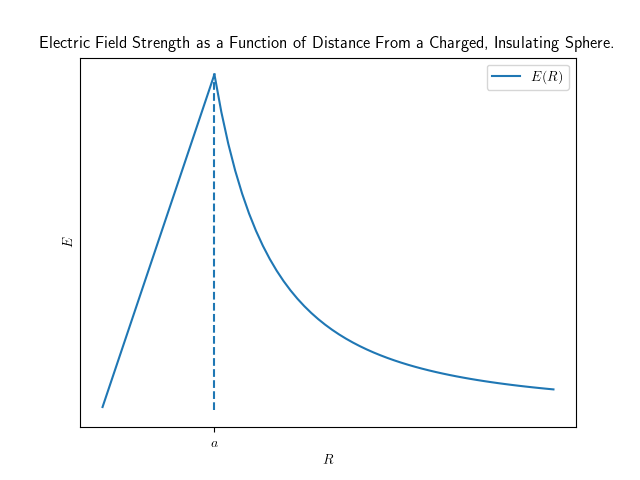
\includegraphics[scale=0.4]{electric_field_insulating_sphere.png}
            \caption{The electric field strength as a function of distance from the centre of a charged insulating sphere.}
            \label{fig:electric field strength insulating sphere}
        \end{subfigure}
        \begin{subfigure}{0.4\textwidth}
            \centering
            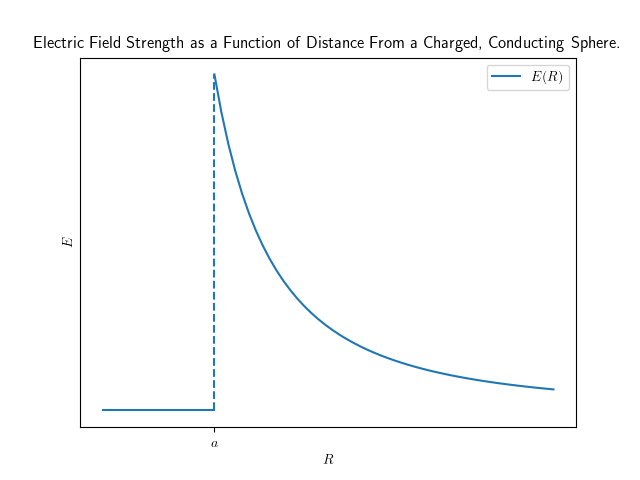
\includegraphics[scale=0.4]{electric_field_conducting_sphere.png}
            \caption{The electric field strength as a function of distance from the centre of a charged conducting sphere.}
            \label{fig:electric field strength conducting sphere}
        \end{subfigure}
        \caption{Electric field strength due to insulating and conducting spheres.}
    \end{figure}
    \subsubsection{Conducting Sphere}
    Consider now the same set up as above but the sphere is made of a conductor.
    Outside of the sphere all of the same logic applies and so for \(R > a\) we have
    \[E(R) = \frac{Q}{4\pi\varepsilon_0}\frac{1}{R^2} = \frac{\rho a^3}{3\varepsilon_0 R^2}.\]
    Inside the sphere the electric field is zero so we have \(E(R) = 0\) for \(R < a\).
    This is plotted in figure~\ref{fig:electric field strength conducting sphere}.
    
    \subsection{Cylindrical Symmetry}
    Take an infinitely long, thin wire with uniform charge density, \(\lambda\).
    We argue that by the symmetry of the situation the electric field must be
    \[\vv{E}(\vv{r}) = E(\rho)\ve{\rho}\]
    where we are working in cylindrical coordinates, \((\rho, \varphi, z)\).
    The argument for this is similar to the spherical case.
    If we place the origin on the wire, this is the only sensible choice for the location of the origin, then we are free to place it anywhere along the wire and we can define \(\varphi = 0\) as any position around the wire.
    This means that the field cannot depend on \(z\) or \(\varphi\) as then the origin position we pick would effect the field strength which is non-physical.
    Similarly if there is a component in the \(\ve{\varphi}\) direction then it must be the same all the way around the cylinder which means that there is a closed loop in the electric field meaning that \(\curl\vv{E} \ne \vv{0}\) which cannot be the case in an electrostatics situation.
    Finally the field can't have a component in the \(\ve{z}\) direction as this would cause motion of charge along the wire which would result in the charge distribution not being uniform.
    Therefore we are left only with dependence on \(\rho\) and a component in the direction \(\ve{\rho}\).
    
    Now construct a Gaussian surface of a cylinder of radius \(\rho\) which shares an axis with the wire.
    The field is always normal to this surface over the curved part so
    \[\vv{E}\cdot\dd{\vv{S}} = E(\rho)\ve{\rho}\cdot\dd{S}\ve{\rho} = E(\rho)\dd{S}.\]
    Over the flat ends of the cylinder the field is parallel to the surface so for the top surface
    \[\vv{E}\cdot\dd{\vv{S}} = E(\rho)\ve{\rho}\cdot\dd{S}\ve{z} = 0,\]
    the case of the bottom surface is the same but \(\dd{S}\) is negative.
    From Gauss' law we then have
    \begin{align*}
        \frac{Q_\mathrm{enc}}{\varepsilon_0} &= \oint_A \vv{E}\cdot\dd{\vv{S}}\\
        &= E(\rho)\int_{\mathrm{CSA}}\dd{S}\\
        &= E(\rho)2\pi\rho L
    \end{align*}
    where \(\mathrm{CSA}\) is the curved surface area of the cylinder and \(L\) is the length of the cylinder.
    The charge enclosed is simply \(Q_\mathrm{enc} = \lambda L\) so rearranging the above equation gives us
    \[E(\rho) = \frac{\lambda L}{\varepsilon}\frac{1}{2\pi\rho L} = \frac{\lambda}{2\pi\rho\varepsilon_0}.\]
    This is plotted in figure~\ref{fig:electric field strength of a charged wire}.
    \begin{figure}[ht]
        \centering
        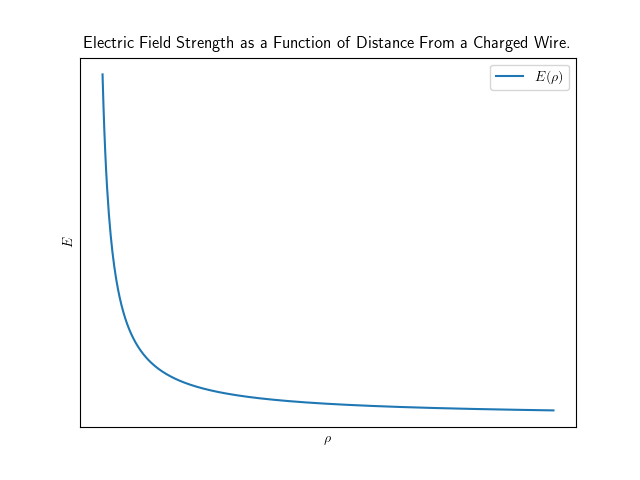
\includegraphics[scale=0.6]{electric_field_wire.png}
        \caption{The electric field strength due to a charged wire.}
        \label{fig:electric field strength of a charged wire}
    \end{figure}
    
    \subsection{Planar Symmetry}
    \subsubsection{Insulating Plane}
    Take an infinite plane with uniform charge density \(\sigma\).
    By symmetry we argue that
    \[\vv{E}(\vv{r}) = E(z)\ve{z}\]
    where we define \(\ve{z}\) as normal to the plane and place the origin in the plane.
    The argument for this is, again, similar to the previous arguments.
    Since we are free to place the origin anywhere in the plane there can be no \(x\) or \(y\) dependence in the field.
    We are also free to rotate the axis around the \(z\) axis which means that any component in the \(\ve{x}\) or \(\ve{y}\) direction must form a complete loop in the electric field which would mean \(\curl\ve{E} \ne \vv{0}\), this is not possible in electrostatics so there must be no \(\ve{x}\) or \(\ve{y}\) components.
    
    We choose a Gaussian surface that is a cylinder of radius \(R\).
    We place it so that its flat faces are parallel to the plane and one is above the plane and the other below.
    As well as this we have both faces the same distance from the plane.
    
    Along the curved surface the field is parallel to the surface so \(\vv{E}\cdot\dd{\vv{S}} = 0\).
    On the top face
    \[\vv{E}\cdot\dd{\vv{S}} = E(z)\ve{z}\cdot\dd{S}\ve{z} = E(z)\dd{S}.\]
    For the bottom case we have \(z < 0\).
    Since we are free to define \(z\)-axis in either direction we must have mirror symmetry in the \((x, y)\)-plane meaning that \(E(-z) = -E(z)\).
    This means that for the bottom face of the cylinder we have
    \[\vv{E}\cdot\dd{\vv{S}} = E(z)\ve{e}\cdot(-\dd{S}\ve{e}) = -E(z)\dd{S}.\]
    However since \(z < 0\) we have \(E(z) = E(-\abs{z}) = -E(\abs{z})\) so
    \[\vv{E}\cdot\dd{\vv{S}} = E(\abs{z})\dd{S}.\]
    This means that the contribution from the two faces is equal to twice the contribution from the top face.
    Applying Gauss' law we have
    \begin{align*}
        \frac{Q_\mathrm{enc}}{\varepsilon_0} &= \oint_A\vv{E}\cdot\dd{\vv{S}}\\
        &= E(z)\int_{2\circ}\dd{S}\\
        &= 2\pi R^2E(z)
    \end{align*}
    where \(2\circ\) is the two circular faces.
    The charge enclosed is \(Q_\mathrm{enc} = \pi R^2\sigma\) so rearranging the above equation gives us
    \[E(z) = \sgn(z)\frac{Q_\mathrm{enc}}{2\pi R^2\varepsilon_0} = \sgn(z)\frac{\pi R^2\sigma}{2\pi R^2\varepsilon_0} = \sgn(z)\frac{\sigma}{2\varepsilon_0},\]
    where
    \[
        \sgn(z) = 
        \begin{cases}
            1, & z > 0,\\
            0, & z = 0,\\
            -1, & z < 0.
        \end{cases}
    \]
    Notice that the only dependence on \(z\) is which side of the plane we are on as that affects the direction of the field.
    The field strength is constant.
    There is a discontinuous jump of \(\sigma/\varepsilon_0\) as we move from one side of the plane to the other.
    This is plotted in figure~\ref{fig:electric field insulated plane}
    \begin{figure}[ht]
        \centering
        \begin{subfigure}{0.4\textwidth}
            \centering
            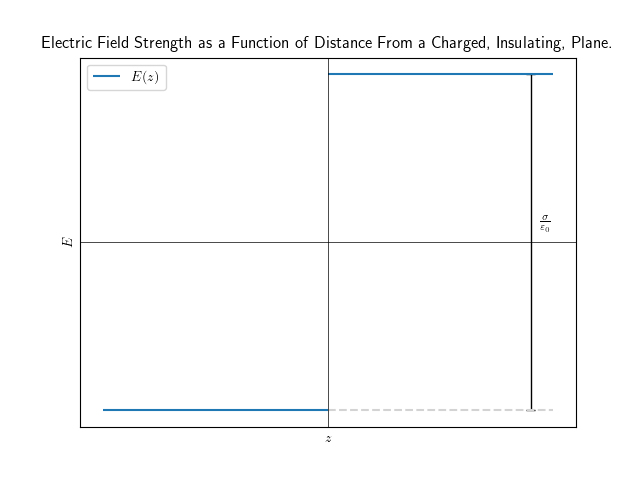
\includegraphics[scale=0.4]{electric_field_insulating_plane.png}
            \caption{Electric field strength as a function of distance from an insulating charged plane.}
            \label{fig:electric field insulated plane}
        \end{subfigure}
        \begin{subfigure}{0.4\textwidth}
            \centering
            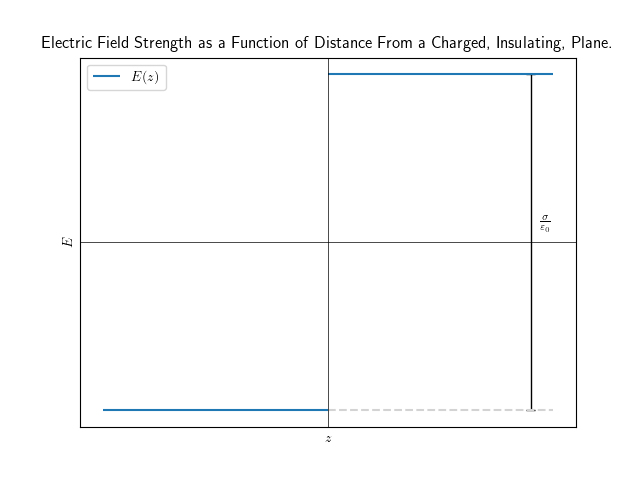
\includegraphics[scale=0.4]{electric_field_insulating_plane.png}
            \caption{Electric field strength as a function of distance from an insulating charged plane.}
            \label{fig:electric field conducting plane}
        \end{subfigure}
        \caption{Electric field strength due to insulating and conducting spheres.}
    \end{figure}
    If instead we have a conducting, charged, plane then the situation is a little different.
    By a conducting plane what we mean is that the plane is the surface of a conductor that continues on below the plane forever.
    The same logic as before works above the plane but now we have that the electric field below the plane is zero as it is inside a conductor.
    Thus
    \begin{align*}
        \frac{Q_\mathrm{enc}}{\varepsilon_0} &= \oint_A\vv{E}\cdot\dd{\vv{S}}\\
        &= E(z)\int_\circ \dd{S},\qquad z > 0\\
        &= E(z)\pi R^2\\
    \end{align*}
    So the electric field strength is
    \[
        E(z) = \begin{cases}
            \frac{\sigma}{\varepsilon_0}, & z > 0,\\
            0, & z \le 0.
        \end{cases}
    \]
    This is plotted in figure~\ref{fig:electric field conducting plane}.
    Note that in both cases there is a discontinuity of \(\sigma/\varepsilon_0\) when passing from one side of the plane to the other.
    
    \section{Poisson's Equation}
    \acrfull{pe} is a \acrfull{pde} of the form
    \[\laplacian\varphi = f\]
    where \(\varphi, f\colon\reals^3\to\reals\).
    The specific case of \(f(\vv{r}) = 0\) gives us
    \[\laplacian\varphi = 0\]
    which is \acrfull{le}.
    This crops up a lot in \acrshort{em} as the electrostatic potential and electric field are connected by
    \[\vv{E} = -\grad V\]
    and the electric field and charge density are related by Gauss' law:
    \[\div\vv{E} = \frac{\rho}{\varepsilon_0}.\]
    Combining these we get
    \[\div(\grad V) = \laplacian V = -\frac{\rho}{\varepsilon_0}.\]
    This simplifies to \acrshort{le} if \(\rho = 0\) everywhere in the region of interest.
    
    The most obvious solution to Laplace's equation is a potential of \(V(\vv{r}) = V_0\) for some constant \(V_0\).
    However as with all \acrshort{pde} there will be a set of \acrfull{bc} and typically \(V(\vv{r}) = V_0\) won't satisfy these \acrshort{bc}.
    Both \acrshort{pe} and \acrshort{le} are among the most important \acrshort{pde} in physics and appear in many scenarios.
    
    \subsection{Properties of Poisson's Equation}
    If \(V(\vv{r})\) is known then it is trivial to compute \(\rho(\vv{r}) = -\varepsilon\laplacian V\) or \(\vv{E}(\vv{r}) = -\grad V\).
    The more likely scenario however is that we know \(\rho(\vv{r})\) and we want to find the electric field.
    The first thing we should attempt should be to use Gauss' law, however this requires high levels of symmetry to be the most useful method.
    Lacking this symmetry the next thing that we can try to do is solve \acrshort{pe} for the potential.
    There is an explicit solution, given by the original definition of the potential:
    \[V(\vv{r}) = \frac{1}{4\pi\varepsilon_0}\int\frac{\rho(\vv{r'})}{\abs{\vv{r} - \vv{r'}}}\dd[3]{r'}.\]
    However this integral often has no analytic solution.
    There are methods for solving it numerically but this is not a numerical methods course so we won't discuss them.
    
    There are two useful properties of \acrshort{pe} that we use to find solutions:
    \begin{enumerate}
        \item The first useful property is linearity.
        If \(V_1\) and \(\rho_1\) satisfy \acrshort{pe} and \(V_2\) and \(\rho_2\) satisfy \acrshort{pe} then \(V_1 + V_2\) and \(\rho_1 + \rho_2\) satisfy \acrshort{pe}.
        That is
        \[\laplacian(V_1 + V_2) = -\frac{1}{\varepsilon_0}(\rho_1 + \rho_2).\]
        This follows trivially from the linearity of \(\laplacian\) as an operator which in turn follows from the linearity of partial derivatives as operators.
        In terms of \acrshort{em} this is just a restatement of the superposition principle.
        One use of this is if we have a shaped charge distribution, \(\rho\), that can be created from simpler shaped charged distributions, \(\rho_i\), then we can find the potential of each individual charge distribution and sum them together to get the potential of the entire charge distribution.
        For example a charged plane with a circular hole can be thought of as a plane without a hole and a charged disc the size of the hole, at the same position but with the opposite charge to the plane over he same area.
        
        \item The second useful property is that the solution to \acrshort{pe} is unique (possibly up to a constant term) for a given set of \acrshort{bc}.
        There are two common ways that \acrshort{bc} are given:
        \begin{itemize}
            \item \(V\) is specified on the boundary -- known as Dirichlet \acrshort{bc}.
            The solution will be unique.
            \item \(\vv{E}\) is specified on the boundary -- known as Neumann \acrshort{bc}.
            The solution will be unique up to a constant term.
        \end{itemize}
    \end{enumerate}
    
    \subsubsection{Proof of Uniqueness}
    \begin{theorem}{Uniqueness of the solution Poisson's Equation}{}
        Consider a region, \(\region\), with boundary, \(\boundary\)\footnote{It is possible that the boundary could be at infinity.}.
        Let \(\rho(\vv{r})\) be specified within \(\region\).
        Let the \acrshort{bc} be given by either
        \begin{enumerate}
            \item \(V\) is specified on \(\boundary\).
            \item \(\vv{E} = -\grad V\) is specified on \(\boundary\).
        \end{enumerate}
        Then any solution of \acrfull{pe},
        \[\laplacian V = -\frac{\rho}{\varepsilon_0},\]
        which satisfies the boundary conditions is unique (up to a constant term in the case of the second set of boundary conditions.)
    \end{theorem}
    \begin{proof}
        Suppose that \(V_1\) and \(V_2\) are two distinct solutions to \(\laplacian V = -\rho/\varepsilon_0\).
        Define \(\psi = V_1 - V_2\).
        Then
        \begin{align*}
            \laplacian \psi &= \laplacian(V_1 - V_2)\\
            &= \laplacian V_1 - \laplacian V_2\\
            &= \rho - \rho\\
            &= 0.
        \end{align*}
        Thus \(\psi\) is a solution to \acrshort{le}.
        Multiplying by \(\psi\) we have
        \[\psi\laplacian\psi = \psi\cdot0 = 0.\]
        Consider the following:
        \[\div(\psi\grad\psi) - (\grad\psi)\cdot(\grad\psi)\]
        Applying the product rule for the divergence of the product of a scalar field and vector field to the first term we get
        \[(\div\psi)\cdot(\div\psi) - \psi(\div(\grad\psi) - (\grad\psi)\cdot(\grad\psi).\]
        The first and last terms cancel and we are left with
        \[\psi(\div(\grad\psi)) = \psi\laplacian\psi = 0.\]
        So the whole term is zero over the whole of \(\region\).
        This means that integrating this term over \(\region\) will also be zero:
        \[\int_\region \div(\psi\grad\psi) - (\grad\psi)\cdot(\grad\psi)\dd{V} = 0.\]
        Applying the divergence theorem to the first term this becomes
        \[\int_\boundary \psi\grad\psi\cdot\dd{\vv{S}} - \int_\region (\grad\psi)\cdot(\grad\psi) \dd{V} = 0.\]
        For either set of boundary conditions the first term is zero.
        The second term is non-negative everywhere as the integrand is the norm of a vector.
        Therefore for the integral to be zero we must have that the integrand is zero.
        The norm of a vector is only zero when that vector is zero therefore
        \[\grad\psi = 0.\]
        This means that \(\psi = V_1 - V_2\) is constant.
        So \(V_1\) and \(V_2\) differ by at most a constant.
        If the boundary conditions were given in terms of \(V\) at \(\boundary\) then we know that \(V_1 = V_2\) at the boundaries so this constant is zero.
    \end{proof}
    
    \begin{example}
        Consider a cavity, \(\region\), in a conductor.
        We claim that if \(\rho = 0\) in the cavity then \(\vv{E} = \vv{0}\) inside the cavity.
        
        The inner surface of the conductor is an equipotential since it is conducting.
        This means that \(V = V_0\) for some constant \(V_0\).
        This is our \acrshort{bc}.
        Inside the cavity we have \(\laplacian V = 0\) since there is no charge.
        Thus we have to solve \acrshort{le} subject to the condition that \(V = V_0\) on the boundary.
        One solution to this is \(V = V_0\) everywhere in \(\region\).
        By the uniqueness theorem above we know that this is the only solution.
        Now we simply compute \(\vv{E} = -\grad V = -\grad V_0 = \vv{0}\).
    \end{example}
    
    \subsection{The Method of Images}
    The method of images is a method for solving \acrshort{pe} by placing `image charges' outside of the region, \(\region\), such that they reproduce the required \acrshort{bc}.
    These charges don't affect \acrshort{pe} inside \(\region\) as they aren't in the region so don't change \(\rho\) in the region.
    However the field that results from the superposition of these image charges as well as any pre-existing charges is the correct solution to \acrshort{pe}.
    
    \begin{example}
        Consider a conducting plane with a point charge, \(Q\), placed a distance \(a\) above the plane.
        What is the potential in the region, \(\region\), above the plane?
        
        The charge density above the plane is
        \[\rho(\vv{r}) = Q\delta(z - a)\delta(x)\delta(y)\]
        where we have placed the origin in the plane directly below the charge and have the \(z\)-axis normal to the plane.
        Our boundary condition is that \(V(x, y, 0) = 0\) as at the plane \(\vv{E} = 0\) so \(V = V_0\) and we choose \(V_0 = 0\) for simplicity.
        
        Unfortunately \(V = V_0\) is not a solution to \acrshort{pe} here as we know that the potential from a point charge falls away as \(1/r\) so at the origin (in the plane directly below the charge) we expect the potential to be \(V = 1/a\) of what it is at the point charge.
        We need to solve
        \[\laplacian V(\vv{r}) = -\frac{\rho(\vv{r})}{\varepsilon_0}.\]
        To do this we can add a homogenous solution, \(V_\text{im}\) to \acrshort{pe}.
        By homogenous here we mean that \(\laplacian V_\text{im} = 0\), i.e. a solution to \acrshort{le}.
        This solution only needs to be homogeneous for \(z \ge 0\) since this is the region of interest.
        We know that the potential due to the point charge is
        \[V_Q(\vv{r}) = \frac{Q}{r\pi\varepsilon_0}\frac{1}{\sqrt{x^2 + y^2 + (z - a)^2}}.\]
        We place an image charge, \(-Q\), at \(z = -a\) which gives us an image potential of
        \[V_\text{im}(\vv{r}) = -\frac{Q}{r\varepsilon_0}\frac{1}{\sqrt{x^2 + y^2 + (z + a)^2}}.\]
        At every point on the plane we have
        \[V_Q + V_\text{im} = \frac{Q}{r\varepsilon_0}\frac{1}{\sqrt{x^2 + y^2 + (0 - a)^2}} - \frac{Q}{r\varepsilon_0}\frac{1}{\sqrt{x^2 + y^2 + (0 + a)^2}} = 0\]
        so the boundary conditions are satisfied.
        Thus \(V = V_Q + V_\text{im}\) is the solution and gives the potential everywhere.
        
        In reality this potential isn't caused by two point charges.
        Rather the real point charge causes the charge density of the plane to become non-uniform in a way that the final potential is as given above.
    \end{example}
    
    \section{Electric Dipoles and Multipoles}
    The motivation behind this section is to study a general, non-trivial, charge distribution, \(\rho(\vv{r})\), and in particular find an approximation of the potential,
    \[V(\vv{r}) = \frac{1}{4\pi\varepsilon_0}\int\frac{\rho(\vv{r'})}{\abs{\vv{r} - \vv{r'}}}\dd[3]{r'},\]
    which applies to points, \(\vv{r}\), far from where \(\rho(\vv{\vv{r'}}) \ne 0\).
    
    \subsection{Electric Dipoles}
    An \define{electric dipole} is formed from two charges, \(\pm q\), fixed distance \(a\) apart.
    The vector from \(q\) to \(-q\) is defined to be \(\vv{a}\).
    The \define{electric dipole moment} is then defined to be \(\vv{p} = q\vv{a}\).
    An electric dipole is shown in figure~\ref{fig:electric dipole}.
    \begin{figure}[ht]
        \centering
        \tikzsetnextfilename{electric-dipole}
        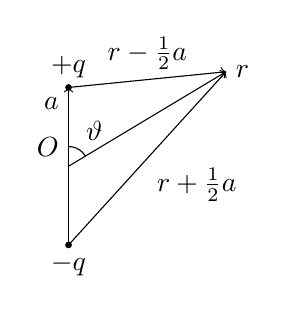
\begin{tikzpicture}
            \draw[fill=black] (0, 1) circle[radius=0.035cm];
            \draw[fill=black] (0, -1) circle[radius=0.035cm];
            \node[above] at (0, 1) {\(+q\)};
            \node[below] at (0, -1) {\(-q\)};
            \node[above left] at (0, 0) {\(O\)};
            \draw[->] (0, -1) -- (0, 1);
            \node[below left] at (0, 1) {\(\vv{a}\)};
            \draw[->] (0, 1) -- (2, 1.2);
            \draw[->] (0, -1) -- (2, 1.2);
            \draw[->] (0, 0) -- (2, 1.2);
            \node[right] at (2, 1.2) {\(\vv{r}\)};
            \begin{scope}
                \clip (0, 0) -- (0, 1) -- (2, 1.2) -- cycle;
                \draw (0, 0) circle[radius=0.25cm];
            \end{scope}
            \node[above right] at (0.1, 0.2) {\(\vartheta\)};
            \node[above] at (1, 1.1) {\(\vv{r} - \frac{1}{2}\vv{a}\)};
            \node[below right] at (1, 0.1) {\(\vv{r} + \frac{1}{2}\vv{a}\)};
        \end{tikzpicture}
        \caption{An electric dipole.}
        \label{fig:electric dipole}
    \end{figure}
    Dipoles like this are important because many molecules, such as \ce{H2O} and \ce{CO} have permanent dipoles and all molecules/atoms acquire an induced dipole in an external field.
    
    \subsubsection{Field of an Electric Dipole}
    The electric potential of an electric dipole is simply the superposition of the potential due to the two point charges:
    \[V(\vv{r}) = \frac{q}{4\pi\varepsilon_0}\left(\frac{1}{r_+} - \frac{1}{r_-}\right)\]
    where 
    \[\vv{r_{\pm}} = \vv{r} \mp \frac{1}{2}\vv{a}.\]
    That is \(\vv{r_\pm}\) is the vector from \(\pm q\) to \(\vv{r}\).
    The next question that we ask is what is the field like for \(r \gg a\)?
    This is known as the far field approximation.
    We can Taylor expand the \(1/r_\pm\) terms in the potential.
    To do this we first note that
    \begin{align*}
        r_\pm^2 &= \vv{r_\pm}\cdot\vv{r_\pm}\\
        &= \left(\vv{r} \mp \frac{1}{2}\vv{a}\right)\cdot\left(\vv{r} \mp \frac{1}{2}\vv{a}\right)\\
        &= r^2 \mp \vv{a}\cdot\vv{r} + \frac{1}{4}a^2\\
        &= r^2 \mp  ar\cos\vartheta + \frac{1}{4}a^2\\
        &= r^2\left(1 \mp \frac{a}{r}\cos\vartheta + \frac{a^2}{4r^2}\right).
    \end{align*}
    Hence
    \[\frac{1}{r_\pm} = \left[r^2\left(1 \mp \frac{a}{r}\cos\vartheta + \frac{a^2}{4r^2}\right)\right]^{-1/2} = \frac{1}{r}\left[\left(1 \mp \frac{a}{r}\cos\vartheta + \frac{a^2}{4r^2}\right)\right]^{-1/2}.\]
    For \(r > a\) this is of the form \((1 + \varepsilon)^p\) with \(\abs{\varepsilon} < 1\) needed to use
    \[(1 + \varepsilon)^p = 1 + p\varepsilon + \order{\varepsilon^2}.\]
    Doing this gives
    \begin{align*}
        \frac{1}{r_\pm} &= \frac{1}{r}\left[1 - \frac{1}{2}\left(\mp\frac{a}{r}\cos\vartheta + \frac{a^2}{4r^2}\right) + \order{\frac{a^2}{r^2}}\right]\\
        &= \frac{1}{r} \pm \frac{a}{2r^2}\cos\vartheta + \order{\frac{a^2}{r^3}}.
    \end{align*}
    Substituting this into the potential gives
    \begin{align*}
        V(\vv{r}) &= \frac{q}{4\pi\varepsilon_0}\left(\frac{1}{r_+} - \frac{1}{r_-}\right)\\
        &\approx \frac{q}{4\pi\varepsilon_0}\left(\frac{1}{r} + \frac{a}{2r^2}\cos\vartheta - \frac{1}{r} + \frac{a}{2r^2}\cos\vartheta\right)\\
        &= \frac{qa\cos\vartheta}{r^2\pi\varepsilon_0}\\
        &= \frac{\vv{p}\cdot\vh{r}}{4\pi\varepsilon_0r^2}.
    \end{align*}
    Notice that this drops off as \(1/r^2\) whereas the potential from a point charge drops off slower as \(1/r\).
    You can think of this as the fact that there are positive and negative charges close together causing parts of the potential to cancel.
    What we have derived here is the far field limit, in that it is only valid for \(r \gg a\).
    It is also known as the `ideal dipole' potential which is what we would get if we too a limit as \(a \to 0\), and \(q\to\infty\) in such a way that \(\vv{p}\) remains constant.
    
    \subsubsection{Dipole Interaction With an External Electric Field}
    The electrostatic energy of a point charge, \(q\), in a potential, \(V\), is \(U = qV\).
    The energy of a dipole is then the superposition of the two point charges:
    \[U_\text{dip} = qV_\text{ext}(\vv{a}/2) - qV_\text{ext}(-\vv{a}/2).\]
    Here \(V_\text{ext}\) is the external potential.
    Taking a Taylor series gives
    \begin{align*}
        U_\text{dip} &\approx q\left[V_\text{ext}(0) + \frac{1}{2}\vv{a}\cdot\grad V_\text{ext}\right] - q\left[V_\text{ext}(0) - \frac{1}{2}\vv{a}\cdot\grad V_\text{ext}\right]\\
        &= q\vv{a}\cdot\grad V_\text{ext}\\
        &= -q\vv{a}\cdot\vv{E_\mathrm{ext}}\\
        &= -p\cdot\vv{E_\mathrm{ext}}
    \end{align*}
    We see that the dipole energy is minimised if \(\vv{p}\) is parallel to \(\vv{E_\mathrm{ext}}\) and the energy is maximised when they are antiparallel.
    The change in energy to change between parallel and antiparallel is
    \[\Delta U = 2p\abs{E_\mathrm{ext}}.\]
    The force experienced by the dipole is
    \[\vv{F} = -\grad U_\text{dip} = \grad(\vv{p\cdot\vv{E_\mathrm{ext}}}).\]
    If \(\vv{E_\mathrm{ext}}\) is a uniform field (doesn't depend on \(\vv{r}\)) then the force is zero.
    This is because the two charges experience equal and opposite forces.
    However there is still a torque because the two charges aren't in the same location.
    This torque acts to align the dipole with \(\vv{E_\mathrm{ext}}\) and is given by:
    \[\vv{\tau} = \frac{1}{2}\vv{a}\times q\vv{E_\mathrm{ext}} - \frac{1}{2}\vv{a}\times(-q\vv{E_\mathrm{ext}}) = \vv{p}\times\vv{E_\mathrm{ext}}.\]
    The work done by the torque to rotate the dipole from aligned with the field to an angle \(\vartheta\) from the field is
    \[W = \int_0^\vartheta \tau\dd{\vartheta} = \int_0^\vartheta qE_\mathrm{ext}\dd{\vartheta} = pE_\mathrm{ext}(1 - \cos\vartheta).\]
    In a non-uniform field the force is generally more complex.
    It acts to move the dipole along the gradient of the field.
    
    \subsection{Multipole Expansion}
    Given a charge distribution \(\rho\) we say that \(\rho\) is bounded inside a region, \(\region\), if, for \(\vv{r}\notin\region\), \(\rho(\vv{r}) = 0\).
    Let \(\rho\) be a charge distribution that is bounded inside the region \(\region\).
    Then from the definition of the potential we know that
    \[V(\vv{r}) = \frac{1}{4\pi\varepsilon_0} \int_\region \frac{\rho(\vv{r'})}{\abs{\vv{r} - \vv{r'}}}\dd[3]{r'}.\]
    This holds for all \(\vv{r}\).
    However if \(\vv{r}\notin\region\), that is \(r \gg r'\), then we can make use of a Taylor expansion.
    Following the same steps as we did for a dipole we see that
    \[\frac{1}{\abs{\vv{r} - \vv{r'}}} = \frac{1}{r}\left[1 - \frac{2\vv{r}\cdot\vv{r'}}{r^2} + \frac{r'^2}{r^2}\right]^{-1/2}.\]
    We now Taylor expand this but keep higher order terms:
    \begin{align*}
        \left[1 - \frac{2\vv{r}\cdot\vv{r'}}{r^2} + \frac{r'^2}{r^2}\right]^{-1/2} &= 1 - \frac{1}{2}\left(-\frac{2\vv{r}\cdot\vv{r'}}{r^2} + \frac{r'^2}{r^2}\right) + \frac{3}{8}\left(-\frac{2\vv{r}\cdot\vv{r'}}{r^2} + \frac{r'^2}{r^2}\right)^2 + \order{\frac{1}{r^3}}\\
        &= 1 + \frac{\vv{r}\cdot\vv{r'}}{r^2} - \frac{1}{2}\frac{r'^2}{r^2} + \frac{3}{2}\frac{(\vv{r}\cdot\vv{r'})^2}{r^4} - \frac{3}{2}\frac{r'^2(\vv{r}\cdot\vv{r'})}{r^4} - \frac{3}{8}\frac{r'^4}{r^4} + \order{\frac{1}{r^3}}\\
        &= 1 + \frac{\vh{r}\cdot\vv{r'}}{r} - \frac{1}{2}\frac{r'^2}{r^2} + \frac{3}{2}\frac{(\vh{r}\cdot\vv{r'})^2}{r^2} - \frac{3}{2}\frac{r'^2(\vh{r}\cdot\vv{r})}{r^3} - \frac{3}{8}\frac{r'^4}{r^4} + \order{\frac{1}{r^3}}
        \shortintertext{keeping only terms of order \(1/r^2\) or lower}
        &\approx 1 + \frac{\vh{r}\cdot\vv{r'}}{r} - \frac{1}{2}\frac{r'^2}{r^2} + \frac{3}{4}\frac{(\vh{r}\cdot\vv{r'})^2}{r^2}\\
        &= 1 + \frac{\vh{r}\cdot\vv{r'}}{r} + \frac{3(\vh{r}\cdot\vv{r'}) - r'^2}{2r^2}
    \end{align*}
    Using this in the definition of the potential gives
    \begin{align*}
        V(\vv{r}) &\approx \frac{1}{4\pi\varepsilon_0}\int_\region \dd[3]{r'} \rho(\vv{r'})\frac{1}{r}\left[1 + \frac{\vh{r}\cdot\vv{r'}}{r} + \frac{3(\vh{r}\cdot\vv{r'}) - r'^2}{2r^2}\right]\\
        &= \frac{1}{4\pi\varepsilon_0}\int_\region \dd[3]{r'} \rho(\vv{r'})\left[\frac{1}{r} + \frac{\vh{r}\cdot\vv{r'}}{r^2} + \frac{3(\vh{r}\cdot\vv{r'}) - r'^2}{2r^3}\right].
    \end{align*}
    Defining some new terms this becomes
    \[V(\vv{r}) \approx \frac{1}{4\pi\varepsilon_0}\frac{Q}{r} + \frac{1}{r\pi\varepsilon_0}\frac{\vh{r}\cdot\vv{P}}{r^2} + \frac{1}{4\pi\varepsilon_0}\frac{1}{r^3}\frac{1}{2}\sum_{i, j}\quadrupole_{ij}\hat{r}_i\hat{r}_j.\]
    Where
    \[Q = \int_\region \dd[3]{r'}\rho(\vv{r'})\]
    is the total charge,
    \[\vv{P} = \int_\region \dd[3]{r'}\vv{r'}\rho(\vv{r'})\]
    is the net dipole moment, a vector with Cartesian components
    \[P_i = \int_\region \dd[3]{r'}r'_i\rho(\vv{r'}),\]
    and \(\quadrupole\) is the quadrupole tensor which has Cartesian components
    \[\quadrupole_{ij} = \int_\region\dd[3]{r'}(3r'_ir'_j - r'^2\delta_{ij})\rho(\vv{r'}).\]
    This representation of \(V\) is the \define{multipole expansion} of \(V\) in Cartesian coordinates.
    The first term is the monopole term.
    It is dominant when \(Q\ne 0\) and reasonably approximates the far field charge distribution as a point charge at the origin.
    When the total charge, \(Q\), is zero then the second term, the dipole term, dominates.
    If this term also vanishes then the third term, the quadrupole term, dominates.
    Note that another way of writing this terms is
    \[\frac{1}{4\pi\varepsilon_0}\frac{1}{r^3}\frac{1}{2} \vh{r}\trans\quadrupole\vh{r} = \frac{1}{4\pi\varepsilon_0}\frac{1}{r^5}\frac{1}{2} \vv{r}\trans\quadrupole\vv{r}.\]
    It is possible to take even more terms of the Taylor series and end up with more terms, however we will stop at three.
    Note that each term of the expansion is a solution to \gls{le} and therefore we can use the method of images with image dipoles and quadrupoles as well as image charges.
    
    \begin{example}\label{exa:dipole moment}
        \begin{figure}[ht]
            \centering
            \tikzsetnextfilename{dipole-example}
            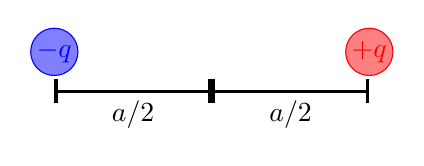
\begin{tikzpicture}
                \draw[color=red, fill=red!50!white] (2, 0) circle[radius=0.3cm];
                \draw[color=blue, fill=blue!50!white] (-2, 0) circle[radius=0.3cm];
                \draw[very thick, |-|] (-2, -0.5) -- (0, -0.5);
                \draw[very thick, |-|] (0, -0.5) -- (2, -0.5);
                \node[red] at (2, 0) {\(+q\)};
                \node[blue] at (-2, 0) {\(-q\)};
                \node[below] at (-1, -0.5) {\(a/2\)};
                \node[below] at (1, -0.5) {\(a/2\)};
            \end{tikzpicture}
            \caption{The dipole setup used in example~\ref{exa:dipole moment}}
        \end{figure}
        A dipole formed of two charges, \(\pm q\), aligned along the \(x\)-axis so that \(q\) is at \((a/2, 0, 0)\) and \(-q\) is at \((-a/2, 0, 0)\) has a charge density given by
        \[\rho(\vv{r}) = q[\delta(x - a/2) - \delta(x + a/2)]\delta(y)\delta(z).\]
        Clearly \(Q = 0\).
        The \(x\) component of the dipole moment is
        \begin{align*}
            P_x &= \int x\rho(\vv{r})\dd{V}\\
            &= q\int x[\delta(x - a/2) - \delta(x + a/2)]\dd{x}\int\delta(y)\dd{y}\int\delta(z)\dd{z}\\
            &= q\frac{a}{2} - q\left(\frac{a}{2}\right)\\
            &= qa.
        \end{align*}
        The \(y\) component is
        \begin{align*}
            P_y &= \int y\rho(\vv{r})\dd{V}\\
            &= \int[\delta(x - a/2) - \delta(x + a/2)]\dd{x}\int y\delta(y)\dd{y}\int \delta(z)\dd{z}\\
            &= 0
        \end{align*}
        since the middle integral is zero.
        Similarly we can show that \(P_z = 0\).
        This means that \(\vv{P} = q\vv{a}\), so we are justified in calling \(\vv{P}\) the dipole moment.
    \end{example}
    \begin{example}\label{exa:quadrupole moment}
        \begin{figure}[ht]
            \centering
            \tikzsetnextfilename{quadrupole-example}
            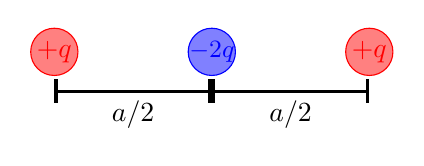
\begin{tikzpicture}
                \draw[color=red, fill=red!50!white] (-2, 0) circle[radius=0.3cm];
                \draw[color=red, fill=red!50!white] (2, 0) circle[radius=0.3cm];
                \draw[color=blue, fill=blue!50!white] (0, 0) circle[radius=0.3cm];
                \node[color=red] at (-2, 0) {\(+q\)};
                \node[color=red] at (2, 0) {\(+q\)};
                \node[color=blue] at (0, 0) {\small\(-2q\)};
                \draw[very thick, |-|] (-2, -0.5) -- (0, -0.5);
                \draw[very thick, |-|] (0, -0.5) -- (2, -0.5);
                \node[below] at (-1, -0.5) {\(a/2\)};
                \node[below] at (1, -0.5) {\(a/2\)};
            \end{tikzpicture}
            \caption{The quadrupole setup used in example~\ref{exa:quadrupole moment}}
        \end{figure}
        Three charges are placed in a line along the \(x\)-axis.
        Two of the charges have charge \(q\) and are at \(\pm a/2\).
        The third charge is at the origin and has charge \(-2q\).
        The charge density is
        \[\rho(\vv{r}) = q[\delta(x - a/2) + \delta(x + a/2) - 2\delta(x)]\delta(y)\delta(z).\]
        Again, \(Q = 0\).
        The \(x\) component of the dipole moment is
        \begin{align*}
            P_x &= \int x\rho(\vv{r})\dd{V}\\
            &= q\int x[\delta(x - a/2) + \delta(x + a/2) - 2\delta(x)]\int\delta(y)\dd{y}\int\delta(z)\dd{z}\\
            &= q\left[\frac{a}{2} - \frac{a}{2} + 0\right]\\
            &= 0
        \end{align*}
        In a similar way to the previous example \(P_y = P_z = 0\).
        Thus the dipole moment vanishes.
        
        Next we calculate the quadrupole moment.
        In general
        \[\quadrupole_{ij} = \int(3x_ix_j - r^2\delta_{ij})\rho(\vv{r})\dd{V}.\]
        The \(\quadrupole_{xx}\) component is
        \begin{align*}
            \quadrupole_{xx} &= \int(3x^2 - r^2)q[\delta(x - a/2) + \delta(x + a/2) - 2\delta(x)]\delta(y) \delta(z)\dd{V}\\
            &= \int(3x^2 - (x^2 + y^2 + z^2))q[\delta(x - a/2) + \delta(x + a/2) - 2\delta(x)]\delta(y) \delta(z)\dd{V}\\
            &= 3q\left(\frac{a}{2}\right)^2 - q\left(\frac{a}{2}\right)^2 + 3q\left(-\frac{a}{2}\right)^2 - q\left(-\frac{a}{2}\right)^2\\
            &= qa^2
        \end{align*}
        Next we will calculate \(\quadrupole_{xy}\):
        \begin{align*}
            \quadrupole_{xy} &= \int 3xyq[\delta(x - a/2) + \delta(x + a/2) - 2\delta(x)]\delta(y) \delta(z)\dd{V}\\
            &= \int 3xq[\delta(x - a/2) + \delta(x + a/2) - 2\delta(x)]\dd{x}\int y\delta(y)\dd{y} \int\delta(z)\dd{z}\\
            &= 0
        \end{align*}
        If we calculated every component we would find that
        \[
            \quadrupole = qa^2
            \begin{pmatrix}
                1 & 0 & 0\\
                0 & -\frac{1}{2} & 0\\
                0 & 0 & -\frac{1}{2}
            \end{pmatrix}
            .
        \]
        We can then approximate the potential as
        \begin{align*}
            V(\vv{r}) &= \frac{1}{8\pi\varepsilon_0} \frac{1}{r^5}\vv{r}\trans\quadrupole\vv{r}\\
            &= \frac{qa^2}{8\pi\varepsilon_0}\frac{1}{r^5}
            \begin{pmatrix}
                x & y & z
            \end{pmatrix}
            \begin{pmatrix}
                1 & 0 & 0\\
                0 & -\frac{1}{2} & 0\\
                0 & 0 & -\frac{1}{2}
            \end{pmatrix}
            \begin{pmatrix}
                x\\ y\\ z
            \end{pmatrix}
            \\
            &= \frac{qa^2}{8\pi\varepsilon_0}\frac{1}{r^5}
            \begin{pmatrix}
                x & y & z
            \end{pmatrix}
            \begin{pmatrix}
                x\\ -\frac{1}{2}y\\ -\frac{1}{2}z
            \end{pmatrix}
            \\
            &= \frac{qa^2}{8\pi\varepsilon_0}\frac{1}{r^5}
            \left[x^2 - \frac{1}{2}(y^2 + z^2)\right].
        \end{align*}
    \end{example}
    \begin{example}\label{exa:quadrupole moment 2}
        \begin{figure}[ht]
            \centering
            \tikzsetnextfilename{quadrupole-example-2}
            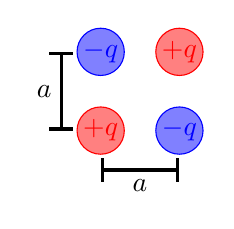
\begin{tikzpicture}
                \draw[color=red, fill=red!50!white] (0, 0) circle[radius=0.3cm];
                \draw[color=blue, fill=blue!50!white] (1, 0) circle[radius=0.3cm];
                \draw[color=blue, fill=blue!50!white] (0, 1) circle[radius=0.3cm];
                \draw[color=red, fill=red!50!white] (1, 1) circle[radius=0.3cm];
                \node[color=red] at (0, 0) {\(+q\)};
                \node[color=blue] at (1, 0) {\(-q\)};
                \node[color=blue] at (0, 1) {\(-q\)};
                \node[color=red] at (1, 1) {\(+q\)};
                \draw[very thick, |-|] (0, -0.5) -- (1, -0.5);
                \draw[very thick, |-|] (-0.5, 0) -- (-0.5, 1);
                \node[below] at (0.5, -0.5) {\(a\)};
                \node[left] at (-0.5, 0.5) {\(a\)};
            \end{tikzpicture}
            \caption{The quadrupole setup used in example~\ref{exa:quadrupole moment 2}}
        \end{figure}
        Four charges \(\pm q\) are placed on the corners of a square in the \((x, y)\)-plane with side length \(a\) with the origin at the centre of the square.
        They are arranged such that diagonally opposite charges have the same sign and charges connected by an edge have opposite signs.
        The charge density is
        
        \begin{multline*}
            \rho(\vv{r}) = q[\delta(x - a/2)\delta(y - a/2) - \delta(x + a/2)\delta(y - a/2) \\- \delta(x - a/2)\delta(y + a/2) + \delta(x + a/2)\delta(y + a/2)]\delta(z).
        \end{multline*}
        Again it can be shown that \(\vv{P} = \vv{0}\) and clearly \(Q = 0\).
        If we calculate the quadrupole components then we find that
        \[
            \quadrupole = qa^2
            \begin{pmatrix}
                0 & 3 & 0\\
                3 & 0 & 0\\
                0 & 0 & -2
            \end{pmatrix}
            .
        \]
        The potential can then be approximated as
        \[V(\vv{r}) = \frac{qa^2}{8\pi\varepsilon_0}\frac{1}{r^5}[6xy - 2z^2].\]
    \end{example}

    \section{Electrostatic Energy and Capacitors}
    \subsection{Electrostatic Energy of a General Charge Distribution}\label{sec:energy electric field}
    If we start with an assembly of \(n - 1\) point charges, \(q_i\), at position \(\vv{r_i}\) then the potential at \(\vv{r}\) is given by the superposition of the potentials of each particle:
    \[V(\vv{r}) = \frac{1}{4\pi\varepsilon_0}\sum_{j=1}^{n-1}\frac{q_i}{\abs{\vv{r} - \vv{r_j}}}.\]
    If we then bring another charge, \(q_n\), from infinity to \(\vv{r_n}\) then the work required to do so is
    \[W_n = q_nV(\vv{r_n}) = \frac{q_n}{\frac{q_n}{4\pi\varepsilon_0}} \sum_{j=1}^{n-1}\frac{q_j}{\abs{\vv{r_n} - \vv{r_j}}}.\]
    We can write out this sum for the first few values of \(n\) to see how it progresses:
    \begin{align*}
        W_1 &= 0\\
        W_2 &= \frac{q_2q_1}{4\pi\varepsilon_0}\frac{1}{\abs{\vv{r_2} - \vv{r_1}}}\\
        W_3 &= \frac{q_3q_1}{4\pi\varepsilon_0}\frac{1}{\abs{\vv{r_3} - \vv{r_1}}} + \frac{q_3q_2}{4\pi\varepsilon_0}\frac{1}{\abs{\vv{r_3} - \vv{r_2}}}
    \end{align*}
    In general the total work required to assemble \(n\) charges, which is the electrostatic energy, \(U_E\), is given by
    \begin{align*}
        U_E &= \sum_{i=1}^{n}W_i\\
        &= \frac{1}{4\pi\varepsilon_0}\sum_{i=1}^{n}\sum_{j=1}^{i - 1}\frac{q_iq_j}{\abs{\vv{r_i} - \vv{r_j}}}\\
        &= \frac{1}{8\pi\varepsilon_0}\sum_{\stackrel{i, j}{i\ne j}}^{n}\frac{q_iq_j}{\abs{\vv{r_i} - \vv{r_j}}}.
    \end{align*}
    In the last step we collapsed two sums into one by noting that a sum over \(i\) and \(j\) with \(i > j\) is equivalent to a sum over \(i\) and \(j\) with \(i \ne j\) except that the second allows for \((i,j) = (2,1)\) and \((i,j)=(1,2)\).
    Due to symmetry the value of both of these terms is the same so we end up double counting the allowed states where \(i > j\) if we include all \(j \ne i\).
    For this reason we have to divide by 2 which explains the factor of \(8\) in the denominator.
    
    In the limit of a continuous charge density, \(\rho\), the electrostatic energy is
    \[U_E = \frac{1}{2}\int\rho(\vv{r})V(\vv{r})\dd[3]{r}.\]
    Using Maxwell's first law this becomes
    \[U_E = \frac{\varepsilon_0}{2}\int V(\vv{r})(\div\vv{E})\dd[3]{r}.\]
    We then use the product rule,
    \[\div(V\vv{E}) = V\div\vv{E} + (\grad V)\cdot\vv{E} = V\div\vv{E} - \vv{E}\cdot\vv{E} = V\div\vv{E} - E^2,\]
    to change the integrand to
    \[U_E = \frac{\varepsilon_0}{2}\int \div[V(\vv{r})\vv{E}(\vv{r})] + E^2\dd[3]{r}.\]
    Splitting the integral at the addition and applying the divergence theorem to the first integral we get
    \[U_E = \frac{\varepsilon_0}{2}\oint_SV(\vv{r})\vv{E}(\vv{r})\cdot\dd{\vv{S}} + \frac{\varepsilon_0}{2}\int E^2\dd[3]{r}.\]
    So far we have made no assumptions about the volume over which our integration occurs.
    This means we are free to pick any boundary, \(S\).
    We choose \(S\) to be at infinity.
    Assuming that our charge distribution is bound we know that outside of the region containing it \(V\) drops of as at least \(1/r\) and \(E\) drops off as at least \(1/r^2\).
    Thus \(VE\) drops of as at least \(1/r^3\).
    The area of the surface however only grows as \(1/r^2\) so the first integral must be zero.
    Thus the internal energy is
    \[U_E = \frac{\varepsilon_0}{2}\int \abs{\vv{E}(\vv{r})}^2\dd[3]{r} = \int u_E \dd[3]{r},\]
    where
    \[u_E = \frac{\varepsilon_0}{2}\abs{\vv{E}(\vv{r})}^2\]
    is the energy density.
    
    Note that this derivation started from a continuous charge distribution.
    This does not apply to point charges.
    If we were to apply it to point charges there are self interaction terms that we would have to exclude.
    We can see this form the point charge equations, if we try to include the interaction of a point charge with itself we get \(\abs{\vv{r_i} - \vv{r_i}} = 0\) so we end up dividing by zero.
    We are now assuming that the integral is over all space, if we wish to only consider a small volume we either require that \(E = 0\) outside of that area or we have to consider the first integral that we reasoned to be zero for an infinite volume.
    As a final warning the electrostatic energy is quadratic in field strength so the superposition principle \emph{does not} apply to energy densities.
    
    \subsection{Capacitors}
    A capacitor comprises of two neighbouring conducting bodies with equal and opposite charges, \(\pm Q\).
    The capacitance is defined to be
    \[C = \frac{Q}{V}\]
    where \(V\) is the potential difference between the two bodies.
    This is well defined as the surfaces of the conductors are equipotentials so it doesn't matter where we select on each conductor to measure the potential difference.
    
    \subsubsection{Parallel Plate Capacitors}
    The simplest capacitor is a parallel plate capacitor where we model the two conductors as thin, infinite, parallel, planes a distance \(d\) apart.
    We can easily calculate the field from the superposition of the fields from two charged planes.
    The set up and electric field from each plate is shown in figure~\ref{fig:parallel plate capacitor electric field}.
    The magnitude of the field from each plate is the same and equal to \(\sigma/2\varepsilon_0\), it is also the same everywhere.
    This is important because it means that between the plates where the fields align the net field is \(\sigma/\varepsilon_0\).
    However outside of the plates the fields are anti-aligned and cancel so the net field is 0.
    \begin{figure}[ht]
        \centering
        \tikzsetnextfilename{parallel-plate-capacitor-field}
        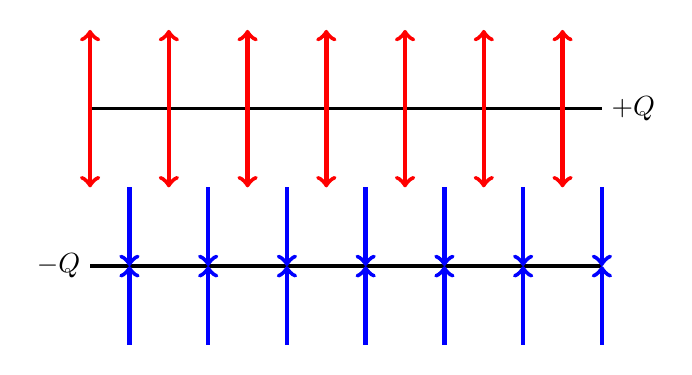
\begin{tikzpicture}
            \draw[very thick] (0, 0) -- (6.5, 0);
            \draw[very thick] (0, 2) -- (6.5, 2);
            \foreach \x in {0,...,6} {
                \begin{scope}[color=red, ultra thick]
                    \draw[->] (\x, 2) -- (\x, 1);
                    \draw[->] (\x, 2) -- (\x, 3);
                \end{scope}
                \begin{scope}[xshift=0.5cm, color=blue, ultra thick]
                    \draw[->] (\x, 1) -- (\x, 0);
                    \draw[->] (\x, -1) -- (\x, 0);
                \end{scope}
            }
            \node[right] at (6.5, 2) {\(+Q\)};
            \node[left] at (0, 0) {\(-Q\)};
        \end{tikzpicture}
        \caption{Parallel plate capacitor electric field.}
        \label{fig:parallel plate capacitor electric field}
    \end{figure}
    The potential difference between the fields is given by
    \[V = -\int_0^d E_z\dd{z} = \frac{\sigma}{\varepsilon_0}d = \frac{Qd}{A\varepsilon_0}\]
    where we have chosen a coordinate system such that \(\ve{z}\) is normal to the plates and points from the negative to the positive plate.
    The origin is also chosen to be in the negative plate.
    The area of each plate is \(A\).
    The capacitance is then given by
    \[C = \frac{Q}{V} = \frac{A\varepsilon_0}{d}.\]
    Notice that the capacitance depends only on the geometry of the plates (their area and the distance between) it is independent of the charge and potential difference.
    It turns out that in general capacitance is a purely geometric property.
    
    We can use the charge distribution to calculate the electrostatic energy of the charged capacitor.
    \begin{align*}
        U_E &= \frac{1}{2}Q(V_1 - V_2)\\
        &= \frac{1}{2}QV\\
        &= \frac{1}{2}\frac{Q^2}{E}
    \end{align*}
    We can also use the fact that the electric field vanishes outside of the plates to calculate the electrostatic energy of the charged capacitor.
    \begin{align*}
        U_E &= \frac{\varepsilon_0}{2}\int E^2\dd[3]{r}\\
        &= \frac{\varepsilon_0}{2} \left(\frac{\sigma}{\varepsilon_0}\right)^2 \int\dd[3]{r}\\
        &= \frac{\sigma^2}{2\varepsilon_0}dA\\
        &= \frac{dQ^2}{2\varepsilon_0A}\\
        &= \frac{1}{2}\frac{Q^2}{E}.
    \end{align*}
    Here we have used that the empty integral is just the volume which in this case since \(E = 0\) outside of the capacitor is just the volume between the plates, \(dA\).
    
    \subsubsection{Edge Effects}
    \textit{This section is non-examinable}
    
    So far we have assume that the plates are infinite and therefore the fields are uniform between the plates.
    However in reality the plates cannot be infinite.
    For a finite sized capacitor the field bulges out of the capacitor and isn't uniform between the plates.
    
    Suppose that instead of infinite planes the capacitor is made from two discs of radius \(R\).
    We can perform an integral over the charge distribution to obtain the potential a height \(z\) above the disc:
    \[V(z) = \frac{1}{4\pi\varepsilon_0}\int_S\frac{\sigma}{(\rho^2 + z^2)^{1/2}}\dd{S}.\]
    In plane polar coordinates \(\dd{S} = \rho\dd{\rho}\dd{\varphi}\) so
    \begin{align*}
        V(z) &= {\sigma}{4\pi\varepsilon_0} \int_{0}^{2\pi} \dd{\varphi} \int_0^R \dd{\rho} \frac{\rho}{(\rho^2 + z^2)^{1/2}}\\
        &= \frac{\sigma}{4\pi\varepsilon_0}2\pi\left[(\rho + z^2)^{1/2}\right]_{\rho=0}^{\rho=R}\\
        &= \frac{\sigma}{2\varepsilon_0}\left[(R^2 + z^2)^{1/2} - z\right].
    \end{align*}
    This means that the \(z\) component of the electric field is
    \[E_z = -\pdv{V}{z} = -\frac{\sigma}{2\varepsilon_0}\left[\frac{z}{(R^2 + z^2)^{1/2}} - 1\right].\]
    This depends on \(z\) so the field is not uniform between the plates.
    There are two interesting limiting cases.
    First \(R \ll z\):
    \begin{align*}
        \vv{E}(R) &= \frac{\sigma}{2\varepsilon_0}\left[1 - \left(1 + \frac{R^2}{z^2}\right)^{-1/2}\right]\ve{z}
        \shortintertext{Taylor expanding the binomial term gives}
        &\approx \frac{\sigma}{2\varepsilon_0}\left[1 - \left(1 - \frac{1}{2}\frac{R^2}{z^2}\right)\right]\ve{z}\\
        &= \frac{\sigma R^2}{4\varepsilon_0 z^2}\ve{z}\\
        &= \frac{Q}{4\pi\varepsilon_0 z^2}\ve{z}
    \end{align*}
    where \(Q = \sigma\pi R^2\) is the total charge.
    We see that in this limit we can essentially view the capacitors as a point charge when we are far enough away that we can approximate it as having no volume.
    
    The other interesting case is when \(R \gg z\).
    In this case the term \(z / (R^2 + z^2)^{-1/2}\approx 0\) so
    \[\vv{E}(R) = \frac{\sigma}{2\varepsilon_0}\ve{z}.\]
    So in the case that the discs are very large they approximate infinite planes.
    It is only when \(R\approx z\) (i.e. \(A\approx d^2\)) that we need to consider the edge effects of the capacitor.
    Fortunately in practice this is rarely necessary.